\chapter{Customized debloating for users with similar feature usage}
\label{chap:dbltr}

\section*{Preamble}
Different users use the same web application differently. 
Based on this intuition, we explored a new approach to debloating, that is, to customize the debloating of web applications, for users with similar usage profile. 
Historically, RBAC (Role Based Access Control) mechanisms have provided the ability for system administrators to allow users to only access the subset of features that they need. 
Unsurprisingly, implementations of RBAC are not free of flaws~\cite{doupe2011fear, dalton2009nemesis, wpfilemanager}. 
Moreover, the over-authorization of users further increases the impact of insider attacks and compromised accounts~\cite{twitterviphack, oktahack}.

To address these challenges, we start by building a real-world ground truth dataset of web application usage patterns in the form of code coverage information through a user study including 60 experienced administrators and developers. 
We then train a classifier that incorporates the source code features to identify users with similar usage patterns and group them together under a dynamically-defined role. 

We design and implement \sys{} which consists of a reverse-proxy that is capable of hooking into the authentication attempts and transparently routing users towards role-specific custom debloated web applications. 
Finally, we evaluate the security benefits of this approach and demonstrate its ability to protect web applications against known CVEs and shrink their attack surface further than the Less is More~\cite{azad2019less}. 
The remainder of this chapter is replicated from the paper titled ``Role Models: Role-based debloating for Web Applications'' which is currently under submission. 

\section*{Role Models: Role-based Debloating for Web Applications}

\subsection*{Abstract}
The process of debloating, i.e., removing unnecessary code and features in software, has become an attractive proposition to managing the ever-expanding attack surface of ever-growing modern applications. Researchers have shown that debloating produces significant security improvements in a variety of application domains including operating systems, libraries, compiled software, and, more recently, web applications. Even though the client/server nature of web applications allows the same backend to serve thousands of users with diverse needs, web applications have been approached monolithically by existing debloating approaches. That is, a feature can be debloated only if none of the users of a web application requires it. Similarly, everyone gets access to the same ``global'' features, whether they need them or not.

Recognizing that different users need access to different features, in this paper we propose role-based debloating for web applications. In this approach, we focus on clustering users with similar usage behavior together and providing them with a custom debloated application that is tailored to their needs. Through a user study with 60 experienced web developers and administrators, we first establish that different users indeed use web applications differently. This data is then used by \sys{}, an automated pipeline for providing tailored debloating based on a user's true requirements. Next to debloating web applications, \sys{} includes a transparent content-delivery mechanism that routes authenticated users to their debloated copies. 
We empirically demonstrate that \sys{} can be 30-80\% more effective than the state-of-the-art in debloating in removing critical vulnerabilities. 

% Introduction
\section{Introduction}

Since the introduction of the World Wide Web, there has been an exponential growth in the number of online websites and web services~\cite{websitestatistics}. 
Our lives are entangled with online services, and companies and governments are hosting their vital infrastructure online. 
Nowadays, companies host their web services behind complex infrastructure that ensures fast and reliable content delivery. 
Moreover, both the quality and the complexity of services have increased drastically over the past decade. 
As the need for more complex online services rose, the development community matured and started building more and more reusable pieces of code. 

% Virtually all popular web development languages and frameworks provide repositories for packages that enhance applications with numerous features and integrations. 
% PHP includes its own package manager called Composer, hosting over 300,000 packages and 3 million versions~\cite{packagist_stats}. 
% NPM, Node.js's package repository, hosts over 1.3 million packages~\cite{npm_statistics}, and Python has Pip which uses PyPI with over 340,000 packages and 3 million versions~\cite{pypi}.

The industry standard in web-development practices switched from writing in-house code from ``scratch'' to the use of professionally developed and maintained third-party modules~\cite{packagiststats, npmstatistics, pypi}. 
Modern web applications commonly incorporate frameworks and packages from public sources to provide routine features such as page management, user authentication, error handling, testing, and logging~\cite{popularphp}. 
Inherent to the use of off-the-shelf software, is the resulting amalgam of features. 
Packages provide a variety of features (e.g., support for multiple database backends) to be useful to as many projects as possible.
At the same time, this added flexibility comes at the price of code bloat. 
Code bloat refers to parts of the application source code that serve no purpose to its users. 
In the example of database APIs, if the website only interacts with a MySQL database, the source code for other database APIs still remains in the application. 
While this may seem benign, flaws in the unused parts of applications can lead to security vulnerabilities~\cite{lessismore, saphire}. 

One line of research called \emph{software debloating} focuses on identifying and neutralizing unused parts of applications. 
Existing systems perform debloating either directly at the source-code level by rewriting the code to remove/block unused code paths~\cite{lessismore, mininode}, or alternatively 
limit the underlying APIs available to each page to reduce the impact of exploits~\cite{saphire}. 
Unlike binaries, when dealing with web-application vulnerabilities, attackers can inject data and execute code, but \emph{cannot} jump to arbitrary instructions within the code. 
Therefore, removing dead code is only of limited benefit for web applications. 
As a result, web application debloating mechanisms commonly remove live code that is deemed as unnecessary based on dynamic code-coverage traces and static analysis. 

One of the main limitations of prior work is the sole focus on one-size-fits-all debloating. 
In such schemes, all users of the web application regardless of their role and access type, receive the same treatment. 
In other words, existing debloating systems produce only one copy of a debloated application to serve all public and authenticated users. 
One may be hopeful that the authentication and access hierarchy within the web applications would prevent access to critical features for untrusted users, yet
this assumption is critically flawed. 
First, not all popular web applications provide fine-grained access control (e.g., phpMyAdmin), and for those that provide access control (e.g., WordPress), the predefined list of available roles may not match the behavioral patterns of users, which can lead to over-authorization. 

Furthermore, access-control flaws where users have access to features that they should not have access to, are commonly found even in popular platforms~\cite{dalton2009nemesis,doupe2011fear}. 
Among other examples, attackers have been able to directly invoke privileged vulnerable modules, which allowed them to fully bypass the authentication and authorization of the main application~\cite{wpfilemanager}. 
Finally, while it is not the main objective of \sys{}, restricting privileged users to well-defined sets of operations can thwart potential insider attacks.

To address the limitations of prior web-application debloating systems
we propose \sys{}, an automatic role-based debloating pipeline that identifies clusters of similar usage patterns among users which can be considered equivalent to an access-control role. 
After identifying the optimal number of clusters (\emph{N}), \sys{} creates \emph{N} debloated copies of the web application tailored to the needs of each subset of users. \sys{} orchestrates the access to these applications through the use of a transparent reverse proxy that captures the successful authentication requests and subsequent authentication cookies to route known users to their custom debloated web applications. 
This process is done without the need to modify target web applications beyond the debloating process, and happens transparently from the perspective of users.

% Public vs. authenticated separation
% Explicit limiting of

\sys{} yields multiple concrete advantages compared to prior schemes of debloating web applications. First, it creates a separation between public and authenticated users which protects web applications even in the face of access-control errors. 
Second, it contains the damage that is possible by a given authenticated user (e.g., due to compromised credentials or client-side attacks) by limiting the attack to the parts of the web application that the user requires for their tasks. 
Lastly, the clustering of users into sets that access differently-debloated web applications, provides a fine-grained access control mechanism, which operates on top of any existing access-control mechanisms and can capture the real needs of users on a feature-by-feature basis. 
For instance, an authenticated WordPress user that only publishes blog posts and replies to comments will receive access to a tailored WordPress application where critical features (e.g., theme modification and plugin installation) are neutralized for that user, yet remain available to other privileged users in the same deployment who rely on them. 

To better understand how the various components of \sys{} work in unison to differentially-debloat and secure web applications, we have prepared the following demonstration. We show a scenario involving a CSRF exploit on phpMyAdmin (CVE-2019-12616) and two users who both visit the same exploit-launching page prepared by an attacker. The video of our demonstration is available online at: \url{https://vimeo.com/652161913} (the video is hosted on a third-party platform to preserve the anonymity of both authors and reviewers).

\noindent Overall, we make the following original contributions:


\begin{itemize}
    \item To back our intuition that different users utilize web applications in different ways, we perform a user study including 60 participants to understand how experienced developers and administrators interact with popular web applications.
    \item We propose \sys{}, an automated web-application debloating and content-delivery system which is capable of reducing the size of applications by up to 70\% and removing as much as 80\% of severe security vulnerabilities beyond the state-of-the-art in web application debloating.
    \item We analyze the security gains and quantify the attack surface reduction of our debloating scheme based on various source code (e.g., line reduction) and security metrics (e.g., CVE reduction, Critical API removal, etc.)
\end{itemize}

To motivate additional research in the area of software debloating, and to ensure reproducibility of our findings, we will be releasing \emph{all} of our software artifacts upon publication of this paper.


% As an example, we can look at a recent vulnerability on WordPress ``File Manager'' plugin~\cite{wpfilemanager}. 
% This popular plugin that has over 800,000 active installations, provides the ability to manage the server's file system to WordPress administrators. 
% While users would assume that this plugin only allows authorized users to interact with the file system, a vulnerability in the implementation allowed even public users to directly upload files without authentication. 
% This attack was possible by sending direct requests to the PHP files of this plugin under \emph{wp-content/plugins/wp-file-manager/lib/files/} to upload malicious files. 
% Unfortunately, existing debloating mechanisms would retain the files for this plugin as long as at least one administrator of that web application used the upload plugin during the trace-collection phase.

% Background
\section{Background}

In this section, we review the topics that will be used as building blocks for the remainder of the chapter. 
First, we discuss the details of debloating web applications based on dynamic code-coverage traces. 
Then, we review several source code metrics that can be used to measure the effectiveness of debloating from the perspective of attack-surface reduction.

\begin{figure}[t]
    \centering
    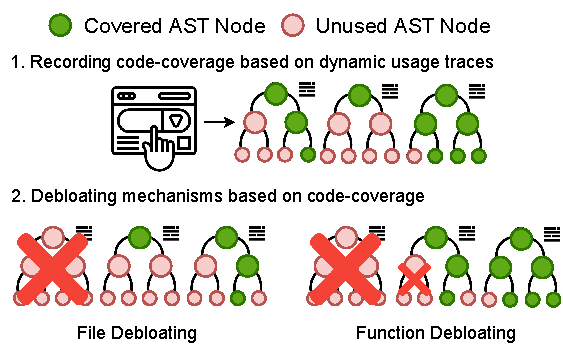
\includegraphics[width=0.75\columnwidth]{figures/dbltr/file_vs_function_debloating.drawio.pdf}
    \caption{File vs Function level debloating based on dynamic code-coverage traces. Root of each AST denotes the entry point of the underlying PHP file. Second layer nodes denote functions, and the leaves are statements inside functions.}
    \label{fig:file_vs_func_debloating}
\end{figure}

\subsection{Debloating based on dynamic usage traces}
Debloating based on dynamic traces for web applications was first introduced in ``Less is More''~\cite{lessismore}, in which we incorporate a set of automation tools and scripts to \emph{simulate} usage behavior while recording the executed server-side files as well as their respective lines.
Figure~\ref{fig:file_vs_func_debloating} represents the two debloating approaches discussed by ``Less is More'' (Chapter~\ref{chap:lim}). 
Based on this code-coverage information (Step 1 in Figure~\ref{fig:file_vs_func_debloating}) ``Less is More'' identifies unused nodes in the Abstract Syntax Tree (AST). 

In ``Less is More'' we discussed two debloating strategies, file-level and function-level debloating. 
In the first approach, file debloating only removes the whole AST of a file, if none of its underlying statements are ever exercised based on the dynamic usage traces. 
Conversely, function debloating is fine-grained and can remove sub-graphs of the AST if it identifies a function with no code-coverage, and therefore, can produce smaller applications with fewer vulnerabilities. 

``Less is More'' incorporates the XDebug PHP module that allows it to record the list of executed PHP file and lines. 
Next step is to configure the web server to start XDebug for each of the running PHP files. 
By configuring XDebug to run for each PHP file invoked by the web server, ``Less is More'' records the list of PHP files and their underlying executed lines and stores them in a database. 
In this work, we follow a similar method to record the code-coverage, and extend ``Less is More'' by looking at \emph{real} user data, and identifying clusters of users that perform similar actions. 

\subsection{Debloating metrics}

Debloating by definition removes or neutralizes parts of the application that users do not require. 
In order to demonstrate the security gains by removing a piece of code, previous work has used several source-code metrics. 

\paragraph{Size reduction} measures how much code was removed through the debloating process. 
McConnell discussed in his work that the size of the code positively correlates with the number of software bugs it contains~\cite{mcconnell2004code}. The reduction in Logical Lines of Code (LLOC) measures the size reduction by counting the number of statements in an application pre-~and post-debloating and is resilient to changes in the syntax and coding style.

\paragraph{Reduction of security vulnerabilities} is another metric that focuses on historic CVEs. 
By mapping public CVEs to the source code of web applications, we can identify whether the vulnerable piece of code is removed by debloating. 
This is a powerful metric as it focuses on real and mostly exploitable vulnerabilities as opposed to proxy variables (such as LLOC) that may or may not result in real vulnerabilities. In terms of downsides, next to the effort required to map vulnerabilities to source code, CVE-reduction is only meaningful in hindsight since it can be used to understand how a debloating system would have performed if an application was debloated \emph{before} the now-known vulnerabilities were discovered. 


\paragraph{Critical API Calls (CAC) reduction} 
PHP applications interact with their environment through the APIs provided by the PHP engine, which are also known as built-in functions. 
These functions expose low-level C API implementations and provide a variety of functionality to perform network, database, and file-system operations. 
Similarly, PHP extensions which are also written in C, expose their functionality through defining new APIs. 

Protecting CACs has received the attention of binary debloating and exploit prevention research in the past. 
Namely, Shredder~\cite{mishra2018shredder}, ROPGuard~\cite{fratric2012ropguard}, and kBouncer~\cite{pappas2012kbouncer} have emphasized the importance of protecting Critical APIs. 
In the realm of web applications, the prior work on taint analysis for vulnerability detection commonly incorporates the list of such critical APIs that attackers can use to execute various types of attacks. 
For instance, attackers can abuse APIs exposed through the MySQLi PHP extension to mount SQL injection attacks. 
Similarly, the exploitation of file-system APIs can lead to arbitrary file-write attacks. 
Therefore, reducing the access of attackers to such functions through debloating provides tangible security benefits. The RIPS tool by Dahse et al. provided a comprehensive list of Critical APIs, which were treated as sinks for PHP taint analysis~\cite{dahse2010rips}. 
We incorporate the 205 sinks from RIPS and measure the removal of such critical API calls (CACs) from the debloated web applications. 

We categorize the sensitive sinks from RIPS into four main groups. \textbf{Code Execution APIs} are those which can be used to directly, or indirectly run code or change the control flow of the application (e.g., call an arbitrary function). 
Next on this list are \textbf{File System APIs} which enable interactions with the file system, such as, deletion and file manipulation and can be abused to take over an application by overwriting files, overriding credentials, and removing sensitive configuration files. 
\textbf{Information Disclosure} functions can be abused by attackers to expose sensitive information from the web application or its host operating system. 
Lastly, for APIs that do not clearly belong to one of the aforementioned categories, we list them under \textbf{Other}. 
This group of critical APIs may allow attackers to conduct malicious actions, such as, sending spam emails, or evading authentication by changing environment variables. 
Next, we look at some examples from each of these categories of critical APIs: 

\begin{itemize}
    \item \textbf{Code Execution APIs:} Consist of OS Shell command execution (e.g., \texttt{exec}, \texttt{passthru}, \texttt{popen}, etc.) PHP code execution (e.g., \texttt{eval}, \texttt{assert}, etc.) and Callbacks (e.g., \texttt{call\_user\_func, array\_map}, etc.)
    \item \textbf{File System APIs :} Consist of functions such as \texttt{fopen}, \texttt{file\_put\_contents}, and \texttt{rename}.
    \item \textbf{Information Disclosure APIs:} Include functions that can leak sensitive information from the web server environment such as \texttt{getenv}, \texttt{get\_current\_user}, and \texttt{phpinfo}.
    \item \textbf{Other APIs:} This group consists of miscellaneous critical APIs such as \texttt{extract}, \texttt{putenv}, \texttt{mail}, etc.
\end{itemize}

The full list of CACs used in this work is available in the Appendix under Table~\ref{tab:cacs}.
    
% \paragraph{PHP Object Injection Gadgets}
% Object injection is a vulnerability where user-controlled values reach an \texttt{unserialize} API without proper sanitization. 
% In such cases, attackers can assemble a list of PHP classes that already exist in an application and mount an exploit which commonly leads to arbitrary file writes and even remote code execution. 

% To understand how attackers exploit PHP object injection vulnerabilities, we need to review two PHP concepts, \emph{Autoloaders} and \emph{Magic functions}. 
% \emph{Autoloading} is a feature in PHP that allows programmers and package developers to register their modules to automatically be loaded by the PHP engine whenever the program instantiates one of their classes. 
% % Therefore, virtually all modern PHP applications that use third-party packages via \texttt{composer} incorporate an autoloader. 
% This expands the ability of the attackers to instantiate all classes across all third-party packages in a vulnerable PHP application. 

% \emph{Magic functions} are special functions that will be invoked automatically by the PHP engine after certain events. 
% Some of the common examples of magic functions used in object injection gadgets are \texttt{\_\_destruct}, \texttt{\_\_toString}, and \texttt{\_\_wakeup}, that are invoked whenever a class is destroyed, converted to a string, or unserialized. 
% % Magic functions sometimes perform sensitive operations, such as, a class destructor performing clean up actions by removing the temporary files generated by that class. 

% In the case of object-injection attacks, the attacker can abuse the code in the existing classes in their target web applications. 
% Since attackers cannot divert the control flow directly by calling arbitrary functions from the injected classes, they rely on specific functions (e.g., class destructors) to piece-together exploit payloads which are called ``gadgets.'' 
% % In the example of destructors removing temporary files, attackers can overwrite the list of these files in the class variable with other sensitive files in the application and force the application to remove them. 

% %Similarly, if the application includes a class with a call to a code execution API (\texttt{include, eval, exec}, etc.) in one of its magic functions, the attackers can abuse this function to run arbitrary code. 

% In this work, we incorporate the list of publicly reported gadgets by PHPGGC~\cite{PHPGGC}. 
% This tool includes a repository of gadget chains within popular third-party packages. 
% Therefore, if a vulnerable application makes use of any of these packages, attackers can inject one of the gadget chains from PHPGGC to gain RCE (Remote Code Execution), write to arbitrary files or interact with the database. 
% PHPGGC does not provide a comprehensive list of gadgets for all packages and all classes in our target web applications. 
% Nevertheless, this approach which is also incorporated in the literature~\cite{lessismore} provides us with a quantitative measure for the reduction in gadget chains after debloating. 

% For each of the web applications in our dataset and their third-party packages, we check for the existence of gadget chains based on the PHPGGC dataset. 
% We then check whether debloating removes these gadgets. 
% For debloated instances where we have removed the gadgets, even if attackers find an object injection vulnerability, they cannot abuse any of the public gadget chains in their exploits. 

% Experimental Design
\section{Experimental Design}

In this section we lay the foundations and discuss the design decisions of our system. 
First we present the details of our user study and data collection. 
We then introduce the design concepts behind \sys{}, our automated pipeline for clustering users into debloating sets and assigning each set to a differently-debloated web application.
Figure~\ref{fig:environment_preparation} shows the high level steps including the data collection and clustering, followed by the preparation of the content delivery environment to serve debloated web applications.

\subsection{User Study - Identifying common web application features from the perspective of experienced administrators}

To understand how experienced users interact with web applications, we conduct the following user study. 
We hire our user-study participants by advertising paid projects on popular freelancing platforms, such as, Upwork~\cite{upwork}. 
After reviewing the resumes and interviewing the candidates, we hire experienced freelancers with 2-10 years of expertise on web development and system administration. 
We specifically interviewed candidates who mentioned phpMyAdmin, WordPress, or Magento on their resume. We focused on these web applications since they were used in the ``Less is More'' study of Amin Azad et al.~\cite{lessismore}, allowing us to compare and contrast our findings with theirs. 

The main goal of this user study is to understand which features in the web applications in our dataset are commonly used among developers and administrators, and which features are relatively unpopular, used by only a fraction of administrators.

\subsubsection{User Study Tasks}

\begin{figure}[t]
    \centering
    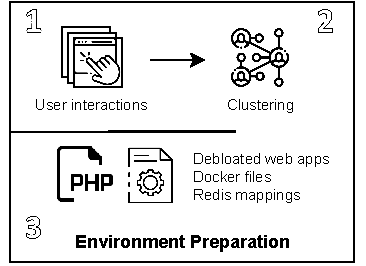
\includegraphics[]{figures/dbltr/EnvironmentPreparation.pdf}
    \caption{During the training phase, we collect user interaction code coverage traces to generate clusters. Based on these clusters, specialized debloated copies of web applications are produced for each cluster.}
    \label{fig:environment_preparation}
\end{figure}

\begin{figure*}[h]
    \centering
    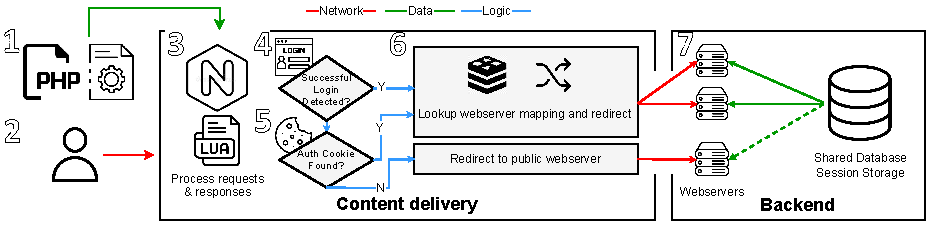
\includegraphics[]{figures/dbltr/RoleModelsFlow.pdf}
    \caption{System Architecture of \sys{}. In Step 1, we provide the debloated web applications and user to cluster mappings to \sys{}'s content delivery module. User requests (2) are processed by \sys{}'s reverse-proxy (Step 3). After identifying the identity of the user (Steps 4-6), \sys{} internally routes the requests to the custom debloated web applications (Step 7).}
	\label{fig:system_architecture}
\end{figure*}

The task description for each project consists of an overview of the user study, the background required to participate, and the expected deliverables. 
Moreover, we included the information about the consent to participate in our study and described the information that we collect (i.e., server-side logs and code-coverage information). 

After interviewing the participants and reviewing their resumes, we hired 20 experts for each web application for a total of 60 experts on phpMyAdmin, WordPress, and Magento. 
We compensate the participants at the rate of \$15 per hour.

During the pilot experiments for the user study, we realized that not every freelancer is familiar with the concept of a user study. 
More importantly, to avoid future disputes, freelancers preferred to work on a predefined list of tasks and deliverables. 

Based on these observations, we defined two milestones for our user study. 
First, we asked our participants to provide a list of web application features that they commonly use in their daily tasks and projects. 
Most of our participants listed both maintenance and administration tasks. 
Among the common tasks, we observed verification of the functionality of the website (e.g., registering as new customers, submitting orders, etc.), maintenance tasks (e.g., backups, import data, etc.) and even search-engine optimization. 

For the second milestone, we asked our participants to spend 1 hour of their time on our instrumented web applications and perform the tasks that they listed earlier. 
This process provided them with the list of deliverables and expectations, and also enabled us to validate their effort on this project. 

For freelancing platforms that provide a time-tracking utility, we use this feature to verify the participation of users together with cross-validating their task report with our code-coverage traces. 
For submissions that did not follow our guidelines (e.g., did not spend enough time, skipped the majority of tasks in the reports, etc.) we would ask the participants to revise their submission. 

\textbf{IRB Approval} Since our experiments involved the assistance of real users, we obtained an Institutional Review Board (IRB) approval for our user study. 
Upon providing thorough details of our tasks and the human interactions, along with the information that we collect from the users, we obtained IRB approval on May 27, 2020. 

\subsubsection{Setup of Web Applications}

To facilitate the setup of web applications for our user study participants, we prepared the following environments:

\begin{itemize}
    \item \textbf{phpMyAdmin:} We provide phpMyAdmin version 5.1.0, with multiple pre-populated databases including a WordPress, and a Magento database.
    \item \textbf{WordPress:} Our setup consists of the version 5.8 of WordPress with an admin account, over 20 blog posts, multiple pages pages, and comments. 
    \item \textbf{Magento:} We setup Magento 2.3.5 and configured the ``Sample data'' package that includes an inventory of over 1,000 products. 
\end{itemize}

Each participant received their own instance with the admin credentials on a unique subdomain. 
We re-create the same environment as ``Less is More'' to collect the usage traces from user interactions in the form of file and line coverage information. 

Through out this user study, we interviewed over 110 individuals, some of whom decided not to participate in our study due to reasons such as non-recurring and short-term nature of our tasks, their busy schedule, etc.
Overall, we spent numerous weeks interviewing our participants and following up with them to ensure the timely delivery of their tasks. The cost of this experiment was approximately \$1,000, most of which was used to pay the administrators in our user study and the remainder to pay for domain names and the hosting of virtual machines on public clouds.

\subsection{Debloating Pipeline}

In this section we describe \sys{}, a dynamic debloating pipeline. 
\sys{} is able to identify web-application users with similar usage profiles (i.e., roles), and create debloated applications that are tailored to the needs of users in each profile. 


Unlike previous one-size-fits-all approaches, application users with specific usage patterns do not need to inherit the whole code-base from other users with vastly different usage behaviors. 
A concrete example of this effect becomes apparent in the usage traces of WordPress. 
Certain administrators focus on the content, and the SEO. 
Therefore, they mostly interact with blog posts and page content, meta tags, and keywords. 
Conversely, another distinct group of administrators focused on changing the appearance of the website by installing new themes, and plugins such as ``Elementor'' that provides an easy interface to modify the appearance of the website. 
In this scenario, by providing the ability to install new plugins to the first group, we are unnecessarily increasing their privileges beyond what they really require. 

For certain web applications, their role-based, access-control mechanisms can limit, to a certain extent, unnecessary capabilities.
Unfortunately many PHP applications that provide administrative features lack this ability (e.g., phpMyAdmin). 
Moreover, the provided roles do not always match the real-world requirements of users. For instance, WordPress comes with only 6 hardcoded roles ranging from Super Admin to Subscriber. 
The benefit of our approach is that we dynamically identify the required web application features based on runtime traces. 

This effect is most significant when applications do not provide fine-grained permission management. 
For instance, using the classic ``single debloated application for all users'' approach, a super admin would share the codebase with data-entry users or even unauthenticated public users. 

Moreover, by clustering users with similar feature usage in the same group, we decrease the likelihood of breaking web application functionality due to removal of code if another user in the same cluster exercised the desired functionality. 
This is in contrast to user-specific debloating where each individual receives their own copy of the target web application based on their exclusive usage patterns. 
We provide a quantitative analysis of this effect in Section~\ref{sec:augmented_coverage}.

\subsubsection{Producing the debloated web applications}

\sys{} extracts the list of exercised files from usage traces. 
PHP file paths and names are effective indicators of the underlying feature corresponding to each file. 
Most commonly, web application source files are partitioned under directories that indicate the feature they implement. 
Moreover, for external dependencies (i.e., composer packages), the file-path includes the name of the module that the files belong to. 

Based on this information, we cluster file paths using the K-means clustering algorithm, into 2 to \emph{N} clusters, with \emph{N} denoting the total number of web application users (in this case, 20).  

\sys{} then produces the following artifacts:
\begin{itemize}
    \item \( \frac{N \times (N - 1)}{2} \) debloated variants of web applications.
    \item Configuration files for the reverse-proxy and the web servers to host the debloated web applications.
    \item Information about the mapping of users to debloating clusters.
\end{itemize}

\subsubsection{Routing users to debloating clusters}

One of the design requirements of \sys{} is seamless user experience. 
Therefore, we incorporate a reverse-proxy that identifies user login information and routes any post-authentication traffic to specialized containers which include debloated variants of the main application customized for the user. 

\sys{}'s reverse-proxy takes a config file for each web application. 
This file informs the proxy of how to identify successful login request-response pairs, the form field that contains the username and the session cookie name to track the user past authentication. 

This information is stored along with the user to web application mappings in an in-memory datastore. 
For authenticated users, the proxy extracts the session cookie, queries the datastore for the web server id for the user and routes the traffic to the appropriate debloated web application. 
From the user's perspective, there is no observable effect while this routing is taking place. Due to the architecture of \sys{}, two users can both be visiting the same URL at the same time, yet accessing radically different (i.e., debloated to match their needs) web applications under the hood. 

\subsubsection{Sharing web application state between web server instances}

Each debloated web application instance is produced from the same source code. 
Nevertheless, the state of each web application depends on the database, cookies, and the session storage. 

In order to keep the state of all web applications synchronized, we connect all of them to the same database instance in the docker environment. 
Moreover, directories that include the session information are mounted as a single volume across all web application instances. 
By sharing this volume, users that authenticate on one copy of the application and are redirected to another debloated instance will maintain their authenticated session cookie. This separation of the session store from web servers is a mainstream principle of scalable web applications allowing requests from the same user to be served by multiple web-server instances~\cite{scalability-book}.
Finally, since web browsers are responsible for maintaining the valid cookies, after routing users to different debloated web application instances served over the same URL, the cookies are automatically transferred along with future requests. 

% Implementation
\section{Implementation}

\dbltr{} consists of multiple data processing, code rewriting, and content delivery steps, making up a full debloating pipeline. 
Initially, our data-analysis step processes the code-coverage traces from web application users and performs the clustering based on the usage data and feature usage. 
Our system incorporates clustering metrics to determine the optimal number of clusters based on code-coverage information, but system operators can decide to modify this configuration based on other post-debloating factors such as LLOC reduction. 

\subsection{Processing the code-coverage information}

For all users of each web application, we extract the list of file and line coverage information. 
Our next task is to identify clusters of code-coverage data based on application usage similarity. 
In order to cluster similar profiles together, we train an unsupervised clustering model based on file names and file paths. 
This decision is based on the intuition that the architecture of popular web applications provides an organic hierarchy of their underlying modules. 

\subsubsection{Vectorizing covered file paths} 
Previously, we argued that file paths and file names are accurate indicators of the underlying feature in the web application based on user interactions and code-coverage traces. 
Based on this observation, we vectorize covered file paths and use TF-IDF algorithm to extract important terms from our corpus of data. 
Throughout this process, we experimentally identified that ignoring common terms that appeared in more than 50\% of the file paths (e.g., \texttt{vendor}, \texttt{wp-admin}, etc.) will yield the best results. 


\subsubsection{Clustering code-coverage information} We use the features returned by the TF-IDF processing in combination with K-Means clustering. 
On one end, we build a single cluster which acts as the baseline for our debloating measurements. 
This cluster which contains the code-coverage of all users resembles the debloating structure of Less is More by Amin Azad et al.~\cite{lessismore}. 
On the other end, we can assign a unique cluster for each user. 
By doing so, each user receives their own uniquely debloated web application which ensures the maximum tailoring of features. 
We argue that the optimal number of clusters lies in between the two extremes, such that the debloating metrics (e.g., code, CVE, and sensitive function call reduction) are optimized while keeping the number of clusters manageable. 

Moreover, as we demonstrate later in Section~\ref{sec:augmented_coverage}, it is beneficial to group users with similar behavior in the same cluster as they will augment each others' code-coverage. 
This aggregation reduces the likelihood of users running into removed features (i.e., features that they did not exercise during the training of the system which were subsequently removed) as other users with similar usage patterns may have already covered the code responsible for the desired feature. 

Web applications sometimes create temporary PHP files for caching purposes. 
Other interactions with the web applications such as installing a new module can also result in the introduction of new PHP code. 
For our debloating scheme, we consider an application at a stable state (i.e., required plugins and modules are already installed prior to debloating). 
Therefore, we perform a cleanup step through which we remove references from code-coverage traces that point to non-existing files in the original version of the applications. 

Our goal in this paper is to demonstrate the debloating performance of popular web applications in their original format. 
Specific to our user study, our cleanup step will essentially remove newly installed modules during the user study experiments, but will keep the code in the original application that enables users to install new modules. 

\begin{figure}[]
    \centering
    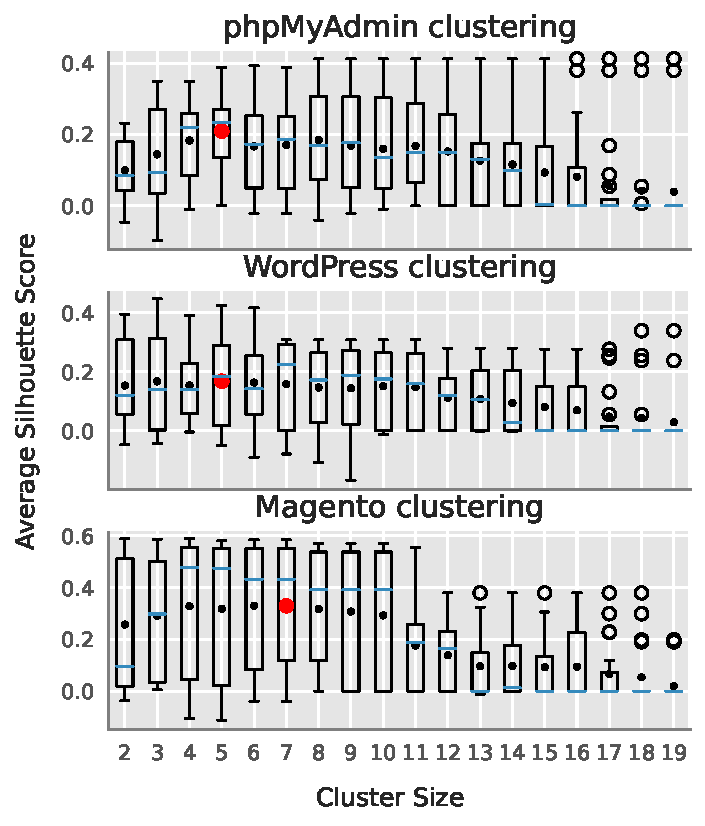
\includegraphics[width=0.50\textwidth]{figures/dbltr/silhouette.pdf}
    \caption{Distribution of Silhouette scores of each cluster. The average score for each cluster is marked with a solid dot and the maximum average is marked with a solid red dot.}
    \label{fig:silhouette_scores}
    \vspace{-1em}
\end{figure}

\subsubsection{Determining the optimal number of clusters} 
\label{sec:num-clusters}

We can determine the optimal number of clusters based on a variety of source code similarity (i.e., file name and path) as well as debloating metrics (i.e., CVE reduction, and CAC reduction). 
\dbltr{} bases its decision on file similarity, concretely file name and path information that is readily available before clustering is performed. 

\dbltr{} then calculates the Silhouette score metric~\cite{kaufman2009finding} for the clusters. 
For each data point, the Silhouette score measures the similarity of the given data point to other points in its own cluster compared to points from other clusters. 
\dbltr{} determines the number of clusters by maximizing the average Silhouette score. 

Figure~\ref{fig:silhouette_scores} depicts the distribution of Silhouette scores based on the cluster size for each of the web applications in our dataset. 
The average score for each cluster size is shown by a solid dot, and optimal cluster size is depicted with a solid red dot. 
Given the ways that the 60 administrators used the evaluated web applications during our user study, the optimal number of clusters are as follows: 5 clusters for phpMyAdmin, 5 for WordPress, and 7 for Magento. 
For certain applications such as Magento, a range of values for the cluster size may be near optimal, in all cases, we selected the number that maximizes the average Silhouette scores.
As the number of clusters increase, we reach an optimal cluster size. 
Beyond this point, by approaching the extreme cluster size (e.g., 19 clusters), we produce many highly-similar small clusters, which reduces the average Silhouette score to close to zero. 

\subsubsection{Debloating the applications} For each cluster, we merge the code-coverage information for all the users of that cluster, and then use the aggregate file and line coverage information to identify unused files and functions and debloat them. 

The process of debloating consists of neutralizing unused files and functions by replacing them with a routine that blocks the further execution of the code. 
This step provides us with \emph{N} copies of the original application, with \emph{N} being the optimal number of clusters determined by \dbltr{}. 
Each debloated cluster caters to the use cases of its underlying users. 
Finally, we calculate the debloating metrics such as size, CVE, and CAC reduction for each cluster. 
We discuss these results in more detail in Section~\ref{sec:debloatingresults}.

\subsection{Content delivery}

The second stage of the \dbltr{} pipeline is responsible for serving the debloated web applications and seamlessly routing users to their underlying debloated web applications. 

\dbltr{} implements a reverse-proxy module based on OpenResty~\cite{openresty}, which is a popular high performance scalable web platform that extends NGINX and provides content manipulation APIs through Lua code. 
This is depicted in Figure~\ref{fig:system_architecture} as step 3. 

We implement the login-detection logic as a Lua module for OpenResty. 
This module is responsible for detecting successful login requests, extracting username and session cookie information, as well as storing and retrieving the user to debloated web application mappings from the data store. 
A high-level representation of the login detection module for phpMyAdmin is depicted in Listing~\ref{lst:lua}.

During the debloating stage, \dbltr{} produces mappings that directs our OpenResty module to redirect users to specific instances of debloated web applications. 
This information is stored in a Redis datastore along with active session-cookie-to-username mappings extracted by the Lua module. 

\definecolor{commentsColor}{rgb}{0.497495, 0.497587, 0.497464}
\begin{lstlisting}[caption=LUA configuration to detect successful logins and extract authentication cookies for phpMyAdmin,label=lst:lua,basicstyle=\footnotesize, float=tp, floatplacement=tbp, language={[5.0]Lua},commentstyle=\color{commentsColor}\textit, numbers=left, xleftmargin=5.0ex, breaklines=true]
-- phpMyAdmin Username extraction
if post_params ~= nil and (string.find(ngx.var.request_uri, "/") or string.find(ngx.var.request_uri, "index.php")) 
  then
    if post_params["pma_username"] ~= nil then
      username = post_params["pma_username"]
    end
end
-- phpMyAdmin Successful login detection
if ngx.var.request_method == "POST" and ngx.var.username ~= "" and ngx.status == 302 then
  -- Successful login detected extract session cookie
  for key, value in pairs(cookies) do
    if string.match(value:lower(), "phpmyadmin") then
      -- Store cookie value in Redis
\end{lstlisting}

For each web application, we provide a configuration file that defines the login endpoint, username form field, and the successful login indicator. 
In the example of phpMyAdmin, successful login is composed of a POST request towards the login endpoint ``/'' or ``index.php'' that receives a 302 HTTP response code which redirects the user to the administration page of the application (Line 2 in Listing~\ref{lst:lua}). 

We extract the username from the POST request with the field name of ``pma\_username'' (Line 4) 
and then verify through the HTTP response code that we detected a successful login (Line 9). Finally, we extract the session cookie named ``phpmyadmin'' (Line 12) and store this user-to-session-cookie mapping in the Redis data store for subsequent requests. 

For subsequent requests containing a valid session cookie, \dbltr{} first queries the username from the data store and then determines the target web server based on the username mapping. 
Steps 4, 5, and 6 in Figure~\ref{fig:system_architecture} depict this process. 
Once the upstream web server is determined, traffic is routed to the corresponding web server. 
Any subsequent log-out requests and timeouts invalidate the session-cookie mapping.
% Debloating Results
\definecolor{commentsColor}{rgb}{0.497495, 0.497587, 0.497464}
\begin{lstlisting}[belowskip=-1em, caption=LUA configuration to detect successful logins and extract authentication cookies for phpMyAdmin,label=lst:lua,basicstyle=\footnotesize, language={[5.0]Lua},commentstyle=\color{commentsColor}\textit, numbers=left, xleftmargin=5.0ex, breaklines=true, float=t, floatplacement=t]
-- phpMyAdmin Username extraction
if post_params ~= nil and (string.find(ngx.var.request_uri, "/") or string.find(ngx.var.request_uri, "index.php")) 
then
    if post_params["pma_username"] ~= nil then
    username = post_params["pma_username"]
    end
end
-- phpMyAdmin Successful login detection
if ngx.var.request_method == "POST" and ngx.var.username ~= "" and ngx.status == 302 then
-- Successful login detected extract session cookie
for key, value in pairs(cookies) do
    if string.match(value:lower(), "phpmyadmin") then
    -- Store cookie value in Redis
\end{lstlisting}

\section{Debloating Results}
\label{sec:debloatingresults}

In this section, we measure the debloating performance of our system and demonstrate its ability to reduce the attack surface of web applications beyond the previous work. 
Next, we compare the debloating results of \dbltr{} and quantify its improvements over the baseline model through source code metrics such as LLOC reduction, as well as security metrics, namely CVE, gadget chain, and CAC reductions. 
% Historically, research papers demonstrated the attack-surface reduction of debloating schemes via the reduction in size of debloated applications.
% Other studies report the removal of historic CVEs and gadget chains as a means to measure the security gains of debloated applications. 
% We extend the existing metrics by measuring and reporting the number of calls to critical API.

% \subsection{Clustering Statistics}
% During our data collection step, we collected the code-coverage data from web application usage from 20 experts for each web application.
% We then clustered their code-coverage information into 1-20 clusters. 
% On one end, the code-coverage information from all users are aggregated in a single cluster. 
% On the other end, all users have their own uniquely debloated web applications that contain only the code that they have interacted with before. 
% While \dbltr{} is capable of providing uniquely debloated web applications for each user, it is beneficial to keep the number of clusters low in order to reduce the complexity of separately maintaining $N$ applications. 

% \subsubsection{Characterizations of \dbltr{} clustering}
% For \dbltr{} debloating clusters, we look at statistics such as number of users in each cluster, as well as the high level roles of each cluster. 

% For the web applications in our dataset, we observe a common list of tasks that are shared among the majority of users. 
% For phpMyAdmin, virtually all users created new database and tables, executed SQL queries, and used the functionality of exporting and importing the database.
% Some users also renamed or modified existing databases, dropped tables, or deleted rows of data. 
% For WordPress, setting up themes and installing custom plugins, and creating new blog posts were among the commonly used features. 
% Finally, for Magento, creating new products, managing product inventory, and modifying prices were the most popular features. 

% \begin{figure}[t]
%     \centering
%     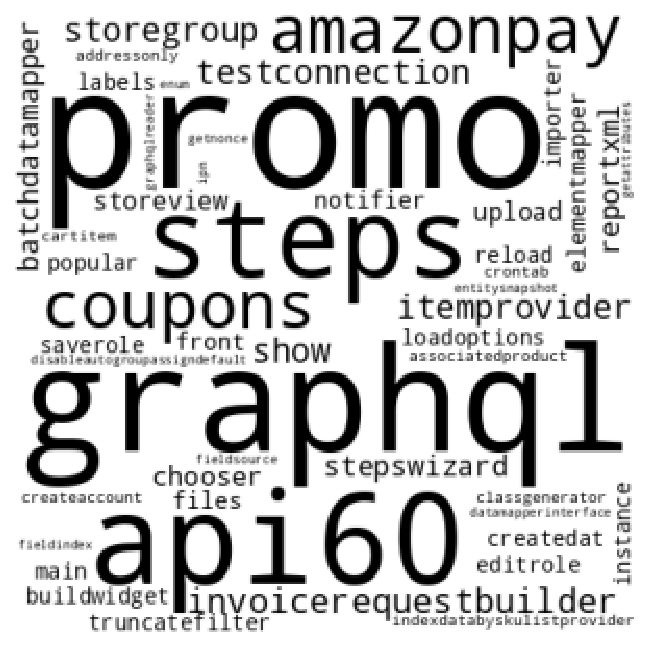
\includegraphics[width=0.5\textwidth]{figures/dbltr/magento_wordcloud.pdf}
%     \caption{Word cloud of important terms for Magento cluster number four}
%     \label{fig:magento_wordcloud}
% \end{figure}

% On the other hand, we observe patterns of feature usage that are unique to a subset of users. 
% Among these user-specific features we observe exporting files with specific file extensions (e.g., CSV), using filters while displaying the query results, and modifying privileges. 
% Similarly, Import/Export, modifying settings such as permalinks, RSS, and WXR are unique to certain clusters among the WordPress users. 
% Finally, for Magento, sales promotions, gifts and shopping cart rules, front end content modification, and sales analytics are among the unique features. 

% We incorporate this observation into our clustering via the max-document-frequency parameter in TF-IDF. 
% This way, we can ignore the common features that are used across all clusters and focus on the unique features when building the clusters. 

% At this step, by looking at the most important terms for each cluster, we can assign a role title to the users of the cluster. 
% Figure~\ref{fig:magento_wordcloud} depicts the word cloud of important terms for a sample cluster of administrators in Magento. 
% Larger font size indicates a higher impact factor based on TF-IDF metric. In general, by analyzing the output of TF-IDF, we can define the following roles for clusters:

% \begin{itemize}
%     \item Mass actions (Delete, Copy, Refresh).
%     \item Invoice, PDF, and Less files.
%     \item Payment methods, Gift cards, and Refunds.
%     \item APIs (GraphQL, XML), Promo, Coupons.
%     \item Index, Cache, Internationalization (i18n).
%     \item Cart, Suggestions, Recommendations.
%     \item Guest purchases, Compare products, Shipping.
% \end{itemize}

\subsection{Debloating results}
%By definition, debloating reduces the effective size of web applications. 
%In this section, we discuss the results of LLOC (Logical Lines of Code), CVE, and CAC (Critical API Call) reduction.

\subsubsection{LLOC Reduction}
 
We measure the reduction in size of web applications in terms of logical lines of code (LLOC), which counts the number of statements in the application source code. 
By reporting the size of the debloated applications in LLOC, we reduce the effects of various syntax and coding styles (i.e., the debloating process changing the code style after rewriting). 

Table~\ref{tab:lloc_reduction} shows the LLOC reduction results of our debloating scheme. 
The numbers are reported in terms of thousands of LLOC. 
The column marked as ``Baseline'' lists the debloating results of combining the code-coverage data of all users together and assigning them to a single role, which is equivalent to prior debloating approaches, such as the one by ``Less is More'' of Amin Azad et al.~\cite{lessismore}.
``\dbltr{}'' shows the LLOC statistics with the optimal number of roles chosen by \dbltr{} for each web application, as discussed in Section~\ref{sec:num-clusters}. 
For \dbltr{} column, we report the size of the role with highest debloated LLOC (Max) and the smallest role with minimum removed LLOC (Min) along with the median. 
The number in the parenthesis for Baseline and \dbltr{} denotes the percentage of LLOC reduction with respect to the size of the original application. 

By comparing the LLOC reduction of Baseline to \dbltr{}, it becomes evident that a one-size-fits-all debloating (i.e., Baseline), exposes certain users and roles to a much larger code-base than they actually require. 
This unnecessary bloat for Baseline debloating can be as high as 30\% of extra LLOC for applications.  
%Nick: This feels like a repetition
%By contrasting the minimum and maximum reduction in \dbltr{} roles, it is evident that in one-size-fits-all debloating schemes certain users would be exposed to a much larger code base than they actually need. 
This unnecessary exposure is most significant for larger web applications such as Magento where certain users inherit up to 90,000 unnecessary LLOC which is 36\% larger---compared to the smallest \dbltr{} role---than what they actually need. 

Moreover, we observe that \emph{all} \dbltr{} roles (including the one with maximum remaining LLOCs) are strictly smaller than the Baseline, meaning that the globally debloated application is still bloated as far as individual users are concerned. 

\begin{table}[t]
    \caption{LLOC reduction of debloated clusters: Numbers are reported in terms of thousands of LLOC. For Baseline, and \dbltr{}, we report the percentage of LLOC reduction compared to the Original application. \dbltr{} columns show the roles with maximum, median and minimum  number of debloated LLOC.}
    \centering
    \adjustbox{max width=\linewidth}{
        \begin{tabular}{|l|l|l|lll|}
            \hline
            \multirow{2}{*}{\textbf{\begin{tabular}[c]{@{}l@{}}Web\\ Application\end{tabular}}} & \multirow{2}{*}{\textbf{Original}} & \multirow{2}{*}{\textbf{Baseline}} & \multicolumn{3}{c|}{\textbf{DBLTR}}                                                  \\ \cline{4-6} 
                                                                                    &                                    &                                    & \multicolumn{1}{l|}{\textbf{Max}} & \multicolumn{1}{l|}{\textbf{Median}} & \textbf{Min} \\ \hline
                phpMyAdmin                                                                          & 155                                & 44 ($\blacktriangledown$72\%)                          & \multicolumn{1}{l|}{32 ($\blacktriangledown$79\%)}    & \multicolumn{1}{l|}{39 ($\blacktriangledown$75\%)}     & 42 ($\blacktriangledown$73\%)     \\ \hline
                WordPress                                                                           & 103                                & 66 ($\blacktriangledown$36\%)                          & \multicolumn{1}{l|}{44 ($\blacktriangledown$57\%)}    & \multicolumn{1}{l|}{54 ($\blacktriangledown$48\%)}    & 64 ($\blacktriangledown$38\%)     \\ \hline
                Magento                                                                             & 1,050                              & 330 ($\blacktriangledown$69\%)                         & \multicolumn{1}{l|}{240 ($\blacktriangledown$77\%)}   & \multicolumn{1}{l|}{270 ($\blacktriangledown$74\%)}   & 326 ($\blacktriangledown$69\%)   \\ \hline
        \end{tabular}
    }
    \label{tab:lloc_reduction}
\end{table}

By comparing the LLOC reduction of Baseline to \dbltr{}, it becomes evident that a one-size-fits-all debloating (i.e., Baseline), exposes certain users and roles to a much larger code-base than they actually require. 
This unnecessary bloat for Baseline debloating can be as high as 30\% of extra LLOC. 
This unnecessary exposure is most significant for larger web applications such as Magento where certain users inherit up to 90,000 unnecessary LLOC which is 37\% larger---compared to the smallest \dbltr{} cluster---than what they actually need. 
Moreover, we observe that \emph{all} \dbltr{} clusters (including the one with maximum LLOCs) are strictly smaller than the Baseline approach, meaning that the globally debloated web application is still bloated as far as individual users are concerned.

\subsubsection{CVE Reduction}

One of the metrics to model the effects of debloating on the security of applications is removal of actual vulnerabilities. 
Historic CVEs provide a good source of information on vulnerabilities and we incorporate a mapping of CVE to source code to identify whether a debloated variant of applications includes the vulnerability or not. 

One of the challenges of this approach is the availability of patch information. 
In order to map a CVE to the vulnerable parts of the source code, we use the data that is available in the form of bug report analysis, Git diffs, and security patches. 
The goal of this step is to identify the files and functions responsible for the vulnerability. 

In our user study, we focused on the latest versions of web applications, so we opted to map all CVEs to these versions. 
In practice, this translates to mapping the location of a CVE to a specific function in a specific file, even if that function is currently patched. 
The purpose of this step is to identify whether the code that contained the vulnerability would have been retained by a debloating approach because it was part of the functionality that the administrators in our user study relied upon.

Some of the web applications in our dataset maintained a stable structure of their source code over time (e.g., WordPress) which makes the process of mapping CVEs from older versions to the recent one straightforward. 
Conversely, phpMyAdmin and Magento changed drastically since their older versions (i.e., Magento version 1.x vs 2.x) and it is not always possible to find the same PHP file/class to perform the mapping. 
Moreover, the developers of phpMyAdmin and WordPress usually acknowledge CVEs in their patches and GitHub commits, whereas for Magento, CVEs are only discussed with minimal details and the patches are released in the form of Major and Minor updates ranging from 500 to 4,000 modifications.

As a result, we mapped 20 CVEs to the source code of phpMyAdmin and WordPress, and mapped 10 recent CVEs to source code of Magento, for a total of 50 mapped CVEs. 
We selected the CVEs with the highest CVSS score, and skipped the ones where the vulnerability or patch information was unavailable. 
The full list of the 50 CVEs that we used in our study along with the information about the \dbltr{} roles such as the number of roles and users that are exposed to each CVE after debloating is available in Table~\ref{tab:cve_details} in the Appendix. 

\begin{figure}[t]
    \centering
    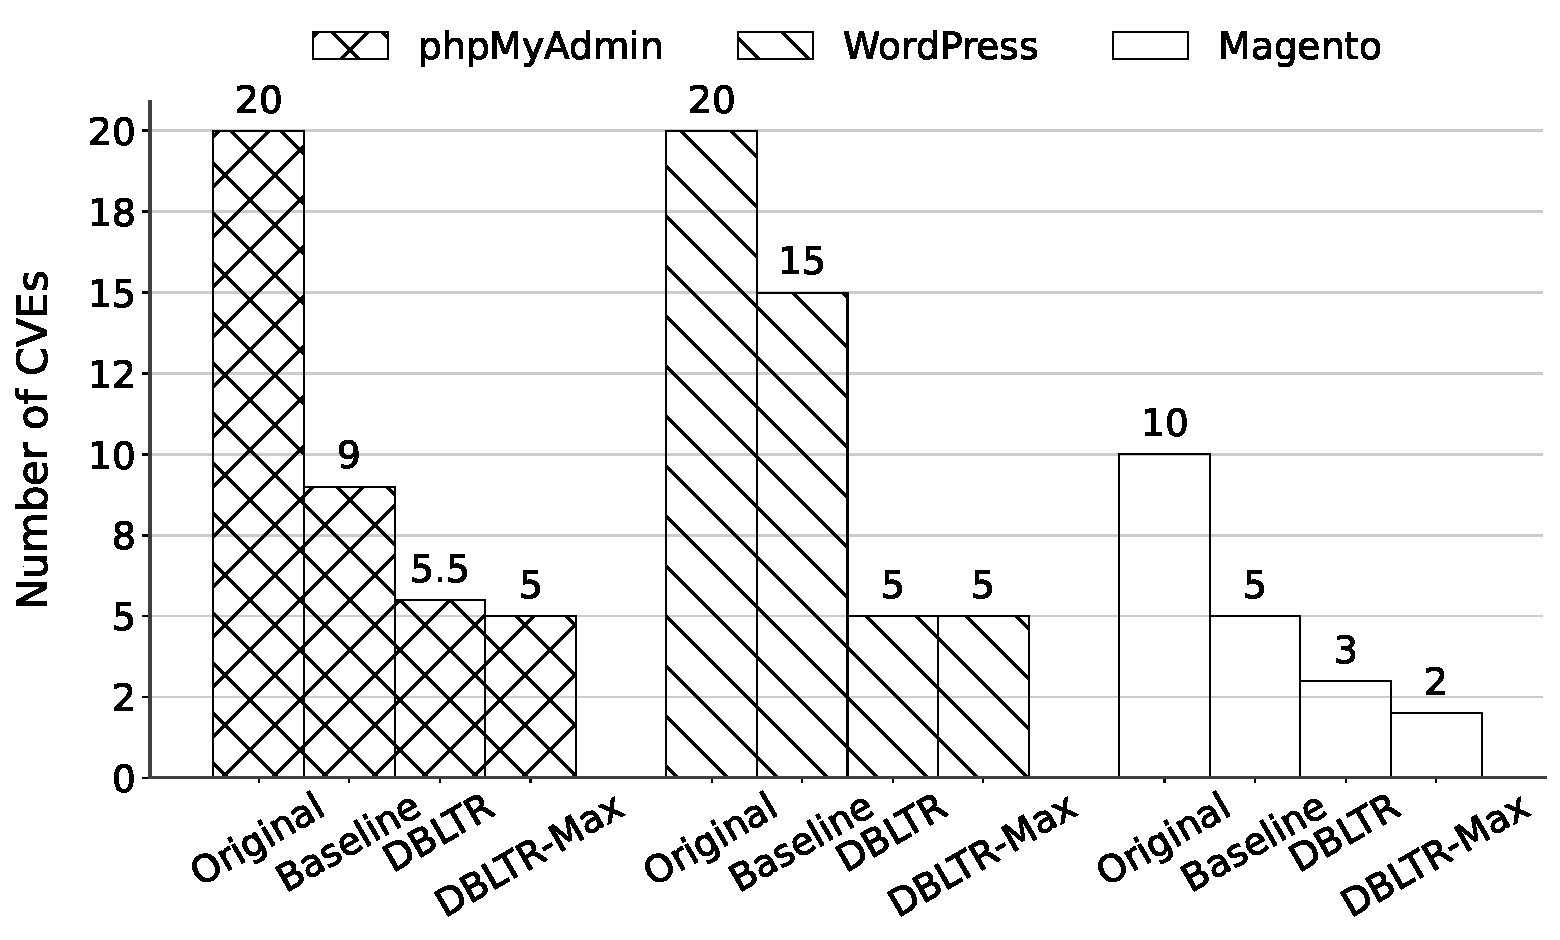
\includegraphics[width=\linewidth]{figures/dbltr/cve_reduction_spectral_bw.pdf}
    \caption{CVE reduction statistics of debloated web applications. ``Original'' represents the total number of mapped CVEs, ``Baseline'' represents the reduction of global debloating, ``DBLTR'' depicts the median reduction across roles, and ``DBLTR-Max'' represents the roles with the highest CVE reduction.}
    \label{fig:cve_reduction}
\end{figure}

Figure~\ref{fig:cve_reduction} depicts the number of CVEs remaining after debloating for each web application. 
The ``\dbltr{}'' bar shows the median CVE reduction across roles, while ``\dbltr{}-Max'' shows the roles with highest CVE reduction representing the maximum protection provided by \dbltr{} for users in those roles. 
For example, for phpMyAdmin we discover that 3/6 roles (accounting for 65\% of users) exposed to the fewest remaining vulnerabilities. 
These roles contained 5 historic CVEs corresponding to 45\% reduction of CVEs compared to the Baseline debloating and 75\% reduction compared to the non-debloated application. 
Similarly, the median number of vulnerabilities among the roles was 5.5 accounting for 40\% reduction compared to the Baseline approach. 
This effect is even more pronounced in WordPress where \dbltr{} reduces the median number of CVEs per role to 4 accounting for a 73\% reduction compared to the 15 CVEs remaining after the Baseline debloating approach. 
Magento exhibits a similar trend of localized debloating gains.

Overall, our results demonstrate that debloating web applications based on clusters of usage-data (i.e., roles) results in significant reduction of severe historic CVEs, compared to prior debloating schemes that could only remove code that was determined to be globally unnecessary for all users of a deployed web application.

\subsubsection{Case Study: phpMyAdmin Database Export Local file Inclusion Vulnerability}

phpMyAdmin version 4.0 is vulnerable to CVE-2013-3240 which resides in the database export functionality. 
This vulnerability allows the attackers to bypass the \texttt{checkParameters} function by sending a specially-crafted variable. 
phpMyAdmin uses this variable to determine the database export file type (e.g., .sql, or .zip) and load the corresponding plugin. 
Malicious users can abuse this flaw to load and execute arbitrary PHP files from the server. 

The export feature in phpMyAdmin is commonly used to backup existing databases and therefore is highly unlikely to be removed by prior global-debloating mechanisms.
Nevertheless, we observed that one of our roles produced by \dbltr{} included four users who did not exercise the export functionality. As a result, \dbltr{} is able to remove this feature from the source code of that specific role, protecting the web application from abuse by these four specific users (including from attackers who compromise their accounts). 

\begin{figure}[t]
    \centering
    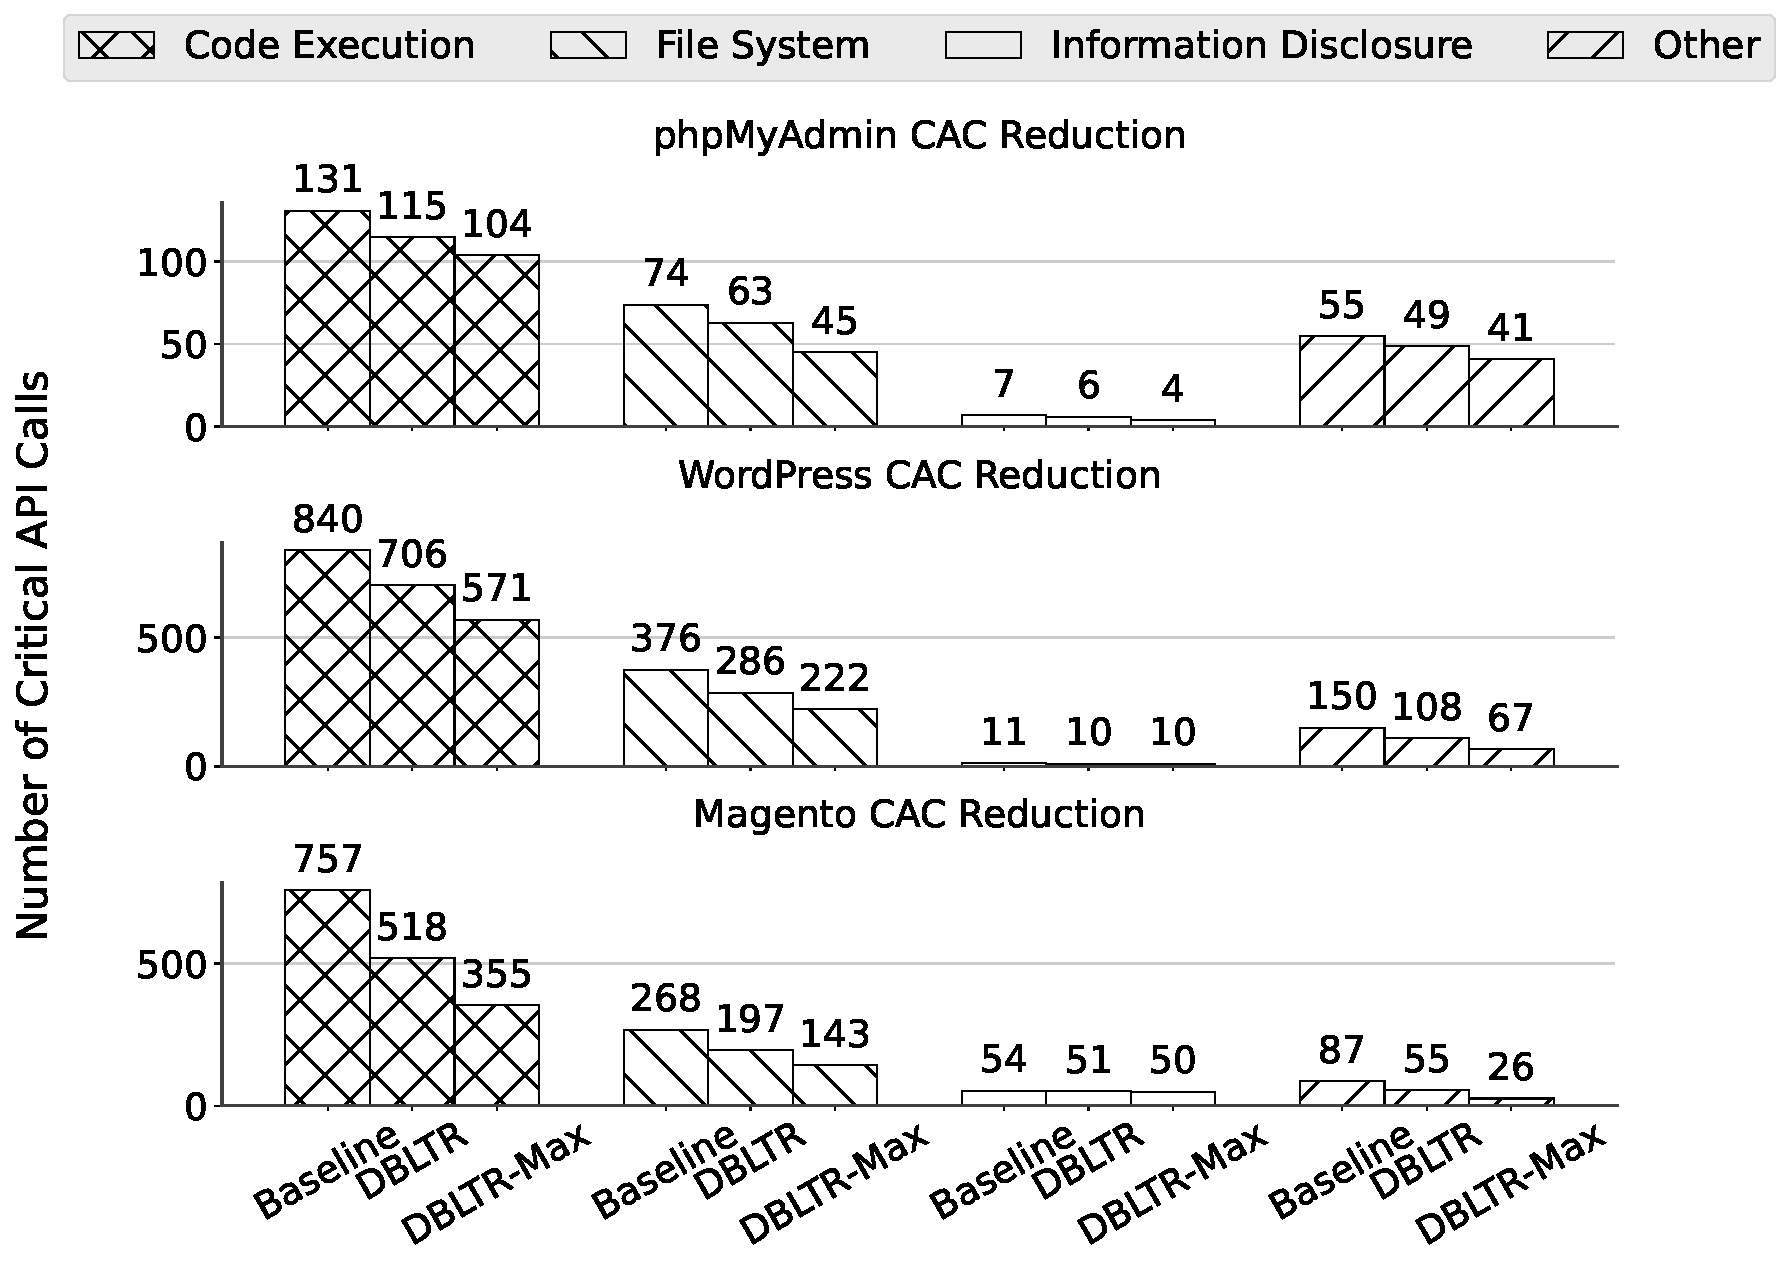
\includegraphics[width=\linewidth]{figures/dbltr/cac_reduction_spectral_bw.pdf}
    \caption{Critical API Call (CAC) reduction after debloating. Baseline represents the global debloating approach where all users are assigned to the same role. \dbltr{} indicates the average reduction across roles.}
    \label{fig:cac_reduction}
\end{figure}

\subsubsection{Critical API Calls Reduction}

Another security metric that we analyze is the reduction in Critical API Calls (CACs). 
Figure~\ref{fig:cac_reduction} depicts the average CAC reduction across all roles. 
The first bar of each group shows the total number of CACs for the Baseline debloating. 
Baseline indicates the reductions in the global debloating scheme where all users are grouped into a single role. 
\dbltr{} bars show the average reduction of CACs based on the optimal number of roles for each web application and \dbltr{}-Max represents the maximum reduction in CACs for a subset of users. 

Across all CAC categories and all web applications, we observe a reduction of 10\% up to 70\% for \dbltr{} debloating. 
This reduction indicates that a sizable number of CACs are in unused parts of the applications. Upon closer inspection of phpMyAdmin results, it becomes evident that 85\% of code execution APIs reside in the external dependencies of the web application, out of which, \dbltr{} removed 12\%-20\%. 
For the larger applications such as Magento, the reduction in Code Execution APIs is more significant where 32\%-53\% of these APIs are removed by \dbltr{}.
Over all categories of CACs, we observe that \dbltr{} removes tens to hundreds of such API calls beyond the Baseline, further protecting web applications from exploits that target these APIs. 

\begin{table}[t]
    \centering
    \caption{PHP Object Injection Gadgets statistics after debloating. Listing number of existing gadgets for Baseline and the percentage of roles in \dbltr{} exposed to those gadgets.}
    \label{tab:poi_gadgets}
    \scalebox{1}{
        \begin{tabular}{|l|l|c|c|c|}
            \hline
            Web Application             & Package & Original & Baseline & \dbltr{} \\ \hline
            \multirow{2}{*}{phpMyAdmin} & Symfony & 2        & 0        & 0     \\ \cline{2-5} 
                                        & TCPDF   & 1        & 1        & 83\%  \\ \hline
            WordPress                   & Generic & 1        & 0        & 0     \\ \hline
            \multirow{3}{*}{Magento}    & Guzzle  & 3        & 2        & 100\%, 0\% \\ \cline{2-5} 
                                        & Magento & 1        & 1        & 14\%  \\ \cline{2-5} 
                                        & Monolog & 6        & 0        & 0     \\ \hline
            \end{tabular}
    }
\end{table}

\subsubsection{PHP Object Injection Gadget Reduction}

To identify existing object injection gadgets in the applications, we incorporate PHPGGC~\cite{PHPGGC}, an open-source project listing available gadget chains for popular composer packages. 
After mapping the list of vulnerable package with those in phpMyAdmin, WordPress, and Magento, we search for the removal of classes and functions used within the gadget chains after debloating. 

Table~\ref{tab:poi_gadgets} lists the packages in each of our web applications with a known gadget chain based on PHPGGC. 
Under the column named ``Original'' we list the number of gadget chains within each package. 
As before, the Baseline column lists the number of gadget chains available after the global debloating (i.e., single role), whereas the \dbltr{} column lists the percentage of roles in \dbltr{} exposed to these gadgets. 

The Symfony package in phpMyAdmin includes 2 known gadget chains that can lead to arbitrary file write and code execution. 
Debloating the application into 1-Cluster (Baseline) as well as \dbltr{} debloating remove these gadgets. 
For TCPDF gadget, while the baseline debloating does not remove it, \dbltr{} protects 17\% of the clusters from object injection exploits using this gadget. 
For WordPress, the baseline debloating strategy removes the existing gadget therefore there are no opportunities for any additional gains by \dbltr{}.

More interestingly, Magento contains 10 known gadget chains. 
For Magento's Guzzle package, we observe that while 2 gadgets are still present in the Baseline debloating, one of the gadget chains is fully removed from all roles.
For the gadget chain within the Magento package itself, only (1/7) 14\% of roles produced by the \dbltr{} contain this gadget, therefore, the majority of users are protected.

Our results confirm the findings of previous work that debloating is a highly effective defense for removing publicly known object injection gadget chains. 
Moreover, we observe that by clustering users into multiple groups, we can further breakdown the availability of gadgets and in certain cases, further complicating the exploitation of object injection vulnerabilities. Under a \dbltr{}-protected deployment, attackers not only need to identify the available gadgets in the target web application to build their exploit chain, but they also have to target \emph{specific} victims who have access to the underlying gadgets used in their exploits. 

% \subsection{Contribution of individual users to the overall code-coverage of clusters}
% \label{sec:augmented_coverage}

% Dynamic code-coverage data precisely models how users interact with web applications. 
% One of the limitations of this modeling is that it overlooks the use cases that it has not seen before. 
% As an example in our dataset, we observed that certain users executed queries that resulted only in a few rows. 
% Therefore, some of the functions within the ``Display Results'' class of phpMyAdmin relating to pagination of results were never invoked. 
% Meanwhile, other users with very similar usage behavior that ended up in the same cluster executed queries that exercised the pagination functions. 
% As a result, all users within this cluster would retain this functionality and can run queries that result in numerous rows.
% In such scenarios, the clustering expands the available features for users with similar usage patterns. 

% To quantify this effect, we look at the contribution of individual users in the cluster compared to the overall cluster code-coverage. 
% For each user, we compare their file and function coverage information with all other users in the same cluster. 
% To identify similar functionality that have been added to the cluster coverage by other users, we look at new lines covered in an already covered file. 
% This modeling captures the effect of exercising new features within an already covered file.
% Moreover, we investigate the inclusion of new files in the overall coverage within an existing module. 
% For this purpose, we closely investigate the source code structure of the web applications in our dataset and identify the directory structure of their internal and external (e.g., composer) packages. 

% \subsubsection{Analyzing module structures} By analyzing the code-base structure of the applications in our dataset, we made the following observations:

% \textbf{phpMyAdmin} uses composer packages. As a result, external dependencies such as Twig, Symfony, Tcpdf, etc. are located under \texttt{vendor/package\_author/package\_name/} directory structure.
% Similarly, phpMyAdmin stores internal modules and classes such as Charsets, Display, Export, etc. under \texttt{libraries/classes/module\_name/}. 
% For phpMyAdmin, we identified 98 external and 23 internal modules.

% \textbf{WordPress} unlike phpMyAdmin, does not use external composer packages. 
% Nevertheless, WordPress modules are split into public and admin sections. 
% Admin modules are located under \texttt{wp-admin/includes/class\_name} and public modules are under \texttt{wp-includes/class\_name}. 
% Some examples of these modules are, PHPMailer, Requests, Rest-API, Widgets, etc.
% Similarly, WordPress themes and plugins have their own unique directory under \texttt{wp-content/themes} and \texttt{wp-content/plugins} directory. 
% For WordPress we identified 23 first-party modules. 

% \textbf{Magento} incorporates multiple first-party and third-party modules via composer. 
% Also, internal modules and classes are located under \texttt{app/code/Magento/module\_name} as well as \texttt{generated/code/module\_name}. 
% From the Magento source code, we identified 493 external and 190 internal modules. 

% Statistics on the code-coverage contribution of clusters to each individual user are available in Table~\ref{tab:augmented_coverage}. 
% Under the column ``\% Files with new coverage'' we report the percentage of total files for which the cluster contributed new lines to the code-coverage of each individual member of that cluster. 
% This number ranges from 15.3\% to 38.3\%, which signifies that a considerable number of functions for each class are included in the final code-coverage by other users in the same cluster. 

% Table~\ref{tab:augmented_coverage} also lists the total number of third-party packages and first-party class modules. 
% Clustering led to inclusion of new files for an average of 29\% to 71\% of packages, and 50\% to 72\% of class modules. 
% On a similar note, these results quantitatively demonstrate that clustering users with similar behavior together leads to inclusion of similar functions, and therefore, reduces the likelihood of removing functions that are actually required by the users. 
% Users who make extensive use of the necessary web-application features cluster together with users with more lightweight usage, allowing the latter to gradually expand their use without breaking the web application due to debloated code. 

% Finally, we look at the number of ``Removed Packages'' for the clusters produced by \dbltr{} in Table~\ref{tab:augmented_coverage}. 
% This column reports the number of packages in the web application where a given percentage of lines are removed after debloating.
% These statistics show that for over half of the packages for phpMyAdmin and Magento, debloating has removed more than 70\% of their lines. 
% In other words, while clustering users with similar behavior together expands their code-coverage of similar features significantly, the debloating procedure is still successfully removing the majority of the code from third-party dependencies, where majority of the bloated code resides~\cite{lessismore}.

\subsection{Performance of \dbltr{}}

We analyze the performance of \dbltr{} from two perspectives, request response time, and server resource utilization. 
Our test setup consists of an HTTP client and the web server. 
The HTTP clients simulate 100 users that send requests in parallel. 
Each client runs in a separate thread and sends batches of 40 requests (average number of requests to load the homepage of WordPress and its resources) towards the main page of WordPress hosted on a remote server. 
This setup simulates the work load for a website with 192,000 daily page views receiving 90 requests-per-second. 
We run each test for five minutes and repeat the tests five times and report the average statistics and remove the outliers. 

For the server setup, our web server hosts a WordPress website and we run each configuration in a containerized environment. 
We run our web servers on a server with 32GBs of RAM, and 32 Cores of Intel Xeon E5-2440 v2 CPUs running Ubuntu 18.04 LTS. 
We test the following setups:

\begin{itemize}
    \item \textbf{Single web server (Apache)} consists of one Apache web server without a reverse-proxy. 
    \item \textbf{Baseline} is made up of an OpenResty reverse proxy and one Apache web server. This setup serves as our baseline. 
    \item \textbf{\dbltr{} setups} expand the baseline setup by including the \dbltr{} modules and consist of one reverse-proxy and 1-50 Apache web servers. Each web server is responsible for the debloated web application for a specific role. This way, we measure the effect of the number of roles on the request response times. Under this setup, each client is assigned to one role in a round-robin fashion.
\end{itemize}

\begin{figure}[]
    \centering
    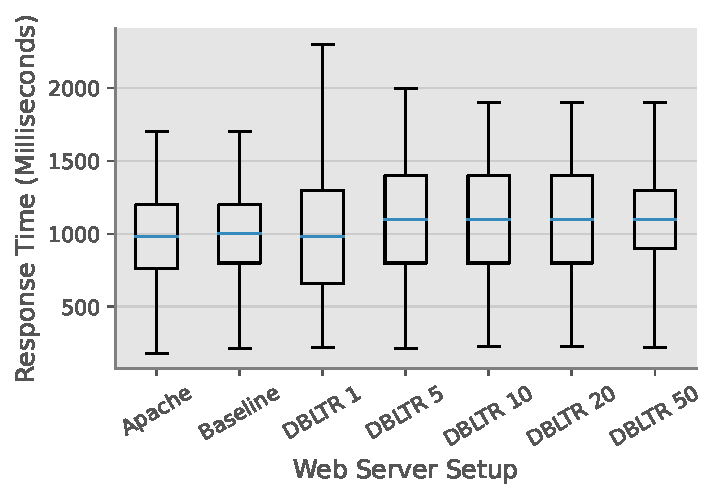
\includegraphics[width=0.8\linewidth]{figures/dbltr/performance.pdf}
    \caption{Distribution of request response time in milliseconds for Apache, Baseline, and \dbltr{} with a varying number of roles (i.e., backed Apache servers).}
    \label{fig:performance}
  \end{figure}

\subsubsection{Request Response Time Statistics}
We measure the request response time statistics from the perspective of our HTTP clients and report them in Figure~\ref{fig:performance}. 
The mere addition of the reverse-proxy (Baseline) increases the median response time of requests by 2\%. 
For \dbltr{}, the overhead from analysis and routing modules results in an average increase of 12\% in the median response time and 15\% increase in the 99th percentile response time. 
Moreover, a higher number of roles reduces the variance in the response times, as evident by the smaller boxes and shorter whiskers from one (DBLTR 1) to fifty roles (DBLTR 50). 

\subsubsection{Resource Utilization}
We measured the CPU and memory utilization of our test setup using the Docker runtime metrics API. 
Table~\ref{tab:performance} reports the resource usage statistics for the web servers and content-delivery (i.e., reverse-proxy) modules. 
Overall, the content-delivery module both in baseline and \dbltr{} setups utilizes 5-6\% of CPU and less than 20~MiB of RAM which is very small compared to the amount of resources utilized by the web server. 
Moreover, across all setups, the CPU utilization of the web server modules remains constant. 
At the same time, increasing the number of roles in \dbltr{} which results in an increase in the number of web servers results in a linear increase in the overall memory utilization. 
During our tests, we observed a 5x increase in overall memory usage of \dbltr{}'s web servers when increasing the number of roles by an order of 50x. 

\paragraph{Disk space utilization} \dbltr{} stores a separate and unique debloated copy of the web applications for each role. 
As a result, the disk utilization overhead of \dbltr{} is proportional to the number of roles. 
While shrinking the disk utilization of \dbltr{} is not a main goal, by definition, the debloating process removes unused lines of code. 
Overall, debloated web applications occupy 5-10\% less disk space. 
While this reduction may be insignificant for smaller web applications, for larger ones such as Magento, debloated web applications on average occupy 100~MB less disk space. 


\begin{table}[]
    \centering
    \caption{Average CPU and Memory utilization of \dbltr{}. \textit{DBLTR N}-Web Servers row shows the range of CPU and Memory utilization for \textit{DBLTR 1} to \textit{DBLTR 50}.}
    \label{tab:performance}
    \adjustbox{max width=\columnwidth}{
    \begin{tabular}{|l|l|l|l|}
    \hline
    \textbf{Setup}                    & \textbf{Module}  & \textbf{Avg CPU} & \textbf{Avg Memory (MiB)} \\ \hline
    Apache                            & Web Server       & 3,117\%              & 2,378                            \\ \hline
    \multirow{2}{*}{Baseline}         & Content-Delivery & 6\%                 & 17                           \\ \cline{2-4} 
                                      & Web Server       & 3057\%              & 2,332                         \\ \hline
    \multirow{2}{*}{\textit{DBLTR N}} & Content-Delivery & 6\%                 & 19                           \\ \cline{2-4} 
                                      & Web Servers      & 2,905-3,072\%      & 2,179-10,374                \\ \hline
    \end{tabular}
    }
\end{table}
% Discussion
\section{Discussion}

In this section we discuss and evaluate possible strategies for handling the addition and removal of users from a \dbltr{}-protected web application. We then review the important takeaways, and finally discuss the limitations of our approach.

\subsection{Addition and Removal of Users} 

The process of assigning a role to new users in RBAC web applications is based on an administrator's discretion regarding the required capabilities of the new users. 
Unlike traditional RBAC roles, \dbltr{} roles are defined dynamically and are unique to each deployment of a web application based on the behavior of its users. 
As a result, assigning new users to existing \dbltr{} roles requires special treatment. 

The conservative approach is to assign new users to a non-debloated web application and record their usage behavior. \dbltr{} can straightforwardly handle this by the mere introduction of a new containerized environment containing that non-debloated web application and a mapping rule assigning the new user to that container. A more aggressive approach is to assign users to a \emph{globally-debloated} web application with the expectation that a newly added user will use features used by at least one existing user of that web application. For both strategies (i.e., conservative and aggressive assignment), administrators can collect usage traces for that new user and eventually invoke \dbltr{} to produce new roles and migrate the new user to a more tailored cluster of users.

To evaluate the latter more aggressive user-assignment strategy, we start by assuming a setup for \dbltr{} where the usage traces for the majority of users have been collected and the roles are produced. This setup resembles an environment (e.g., a company) where the majority of employees were present for the usage-trace collection period and a limited number of new users (e.g., newly-hired employees) are periodically added to this steady-state system. When a new user is added to the system, we use the sum of the code-coverage of all existing users to produce a globally-debloated web application, which still contains a significantly smaller attack-surface compared to the original application. 


To simulate this, we conduct the following leave-one-out experiment: we remove the code-coverage information of each user from the training dataset and create a debloated copy of the web application based on the code-coverage of remaining users (i.e., 19/20 users). 
This globally-debloated web application is strictly larger than any of the role-specific copies of the same application and is equivalent to prior dynamic debloating approaches~\cite{lessismore}. We then simulate the addition of new users by introducing the code-coverage of the user that we left out and measuring false positives, i.e., the files required by that user that are not present in the globally-debloated web application.

\begin{figure}[t]
    \centering
    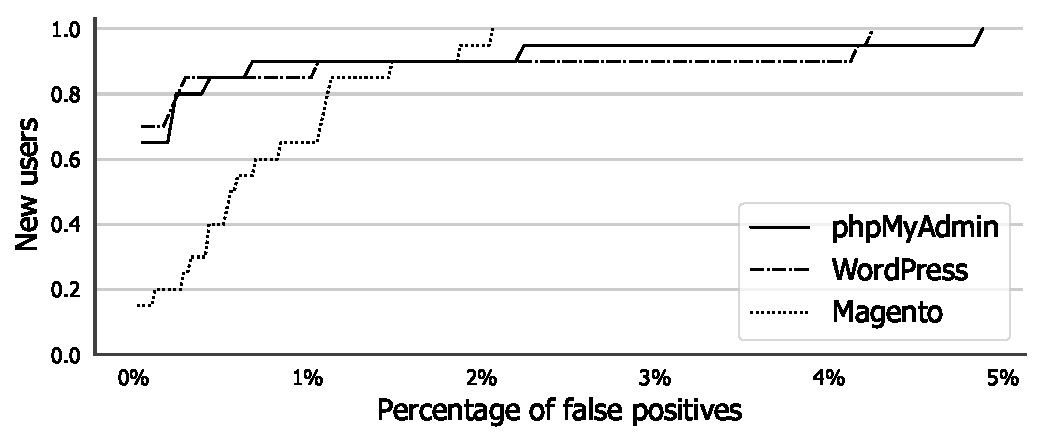
\includegraphics[width=\linewidth]{figures/dbltr/cdf_falsepositives_bw.pdf}
    \caption{CDF of observed false positives from the perspective of new users. The X axis depicts the percentage of false positives (i.e., ratio of the number of missing files compared to total used files by each new user).}
    \label{fig:adding_new_users}
\end{figure}

Figure~\ref{fig:adding_new_users} provides the CDF of false positives (i.e., missing files) when adding new users. 
For phpMyAdmin and WordPress, the majority (60-70\%) of users in the leave-one-out experiment could be added to the ``globally-debloated'' web application without any false positives. 
Likewise, more than 85\% of new users would experience breakage in less than 1\% of the overall files that they interact with. 
For Magento, while most new users assigned to the ``globally-debloated'' web application would experience some breakage, most still fall below the 1\% threshold. 
Overall, across all three web applications in our dataset, even for users with notably unique behavior, we observe less than 5\% of the overall files missing when their usage behavior traces were omitted from the training dataset. 

Looking at the unique behavior of users that led to false positives, in phpMyAdmin, we observe enabling multistep authentication modules, using query explainer features, and creating SQL Views to be the underlying cause (i.e., desired functionality that is unavailable to new users). For WordPress, customizing the RSS feed, using specific text blocks in posts such as text art, and quotes, and using less popular embedding protocols led to false positives under this aggressive user-assignment strategy. Finally, for Magento, various users interacted with unique features.  These features include third-party integrations (e.g., monitoring, marketing, and automation services), PDF invoices, and wish lists. 

Overall, our results show that the modular architecture of \dbltr{} allows it to successfully serve different types of environments. For environments with fixed workloads or where security is prioritized over usability, \dbltr{} can be used to assign new users to a globally-debloated web application. Alternatively, when administrators are unsure about the needs of new users, \dbltr{} can be used to serve the original version of a web application to these users, until enough usage traces are collected to allow \dbltr{} to create new roles and clusters. In either scenario, the security-related debloating benefits of existing users are not in any way compromised when new users are added to a system. In terms of removing users, administrators can merely disable user-role mappings in \dbltr{}'s configurations and optionally delete containers that do not have any roles associated with them.

\subsection{Main Takeaways}

\noindent\textbf{Static roles in web applications are over authorized and administrators only need a subset of the available features:} 
Throughout our user study, we determined that administrators of the same web application use different subsets of the features available to them. 
While in theory, administrators have full access to every feature in the administration panel, in practice only 25\% and 52\% of the lines in the administrative panels of phpMyAdmin and WordPress respectively, were among the commonly exercised features. 
Evidently, the existing authorization mechanisms of these applications aim to offer access to a large variety of features whereas, in reality, administrators only need a subset of them. 
\dbltr{} builds an accurate list of required features and enforces the principle of least privilege via debloating. 

\noindent\textbf{One-size-fits-all debloating still produces bloated web applications:} 
As demonstrated by this work and the literature, debloating web applications is highly effective in reducing the attack-surface of web applications by removing unused features and their underlying vulnerabilities. 

The global debloating approach explored by the prior work produces one debloated web application which as demonstrated by our analysis, can contain as much as 29\% extra LLOC compared to what users actually need. 
In this work, we integrated \dbltr{} with a dynamic debloating scheme and demonstrated that \dbltr{} can provide improvements across all debloating metrics. 
We demonstrated that in the case of global debloating, users in at least half of the roles would be provided with larger web applications containing 5,000-60,000 more lines of code than required, and exposed to 40\%-70\% more CVEs.

% \noindent\textbf{Clustering users with similar behavior together reduces the likelihood of broken features:} 
% In Table~\ref{tab:augmented_coverage} we reported that 15-38\% of files covered by each user in a cluster had new functions covered by other users in the same cluster. 
% Moreover, 29-71\% of third-party packages in a cluster and more than half of internal modules had new files added to the coverage from the perspective of each member of the clusters. 
% Both of these results show that clustering users based on their feature usage can produce debloated applications with shrunk attack-surface, while reducing the likelihood of debloating useful features due to overfitting to the specific usage traces of individual users. 

\noindent\textbf{\dbltr{} provides a content delivery environment for debloated web applications:} 
One of the main contributions of our work is our content delivery pipeline which reduces the need for modifications and customizations to target web applications, while keeping the debloating platform entirely invisible to web application users.

\subsection{Limitations} 

%Our work comes with some limitations that we discuss in this section. 

\noindent\textbf{Debloating statistics: }
As part of our analysis on the security benefits of debloating, we mapped 50 CVEs to the source code of our applications. 
We used recent versions of three popular web applications for our user study and debloating.
By the time they become public, CVEs are either already patched or will be patched soon. 
Therefore, we mapped historic CVEs to the patched functions within the new web applications. 
As a result, our reports on CVE reduction indicate the removal of a feature in a more recent version of web application compared to the original version that included the actual vulnerability. This was a ``necessary evil'' since we could not rely on users perfectly replicating their workloads across multiple versions of the same web applications where the original vulnerabilities resided.

\noindent\textbf{Usage behavior modeling: }
Our debloating reports are based on the code-coverage that we collected during our user study. Using our domain knowledge, we have established that the collected dataset is a representative sample of web-application use in the real world. At the same time, different deployments of web applications may be used differently and therefore be debloated differently. Regardless of the degree of use, \dbltr{} can offer concrete security advantages to any existing or future end-to-end debloating strategy by automatically removing code that is not globally required by all users of a given deployment and clustering users to their appropriately-debloated codebase.

\noindent\textbf{Applications with a public interface: }
As depicted in Figure~\ref{fig:system_architecture}, \dbltr{} routes unauthenticated requests towards a ``public'' profile of the debloated web application. 
This profile includes the code for user authentication as well as any other code required for public unauthenticated users. 

For administrative applications that are behind an authentication wall, producing a public profile is straightforward. 
In the example of phpMyAdmin, we only need to perform successful and failed login attempts to generate the baseline code-coverage and debloat the application to produce the public debloated profile. 
For other applications such as WordPress and Magento, this step is more involved. 
First, we would remove all the files that are only available to the administrators, for the WordPress and Magento, this constitutes of removing administrator directories (e.g., \emph{wp-admin} for WordPress and \emph{module-backend} directory for Magento).
Next, we need to only retain the features and modules that are available to public users. 
Therefore, we need to record the code-coverage of unauthenticated users with benign behavior. 

One of the main benefits of our role-based debloating is the removal of features that are not limited by the authentication and authorization boundaries of web applications. 
If attackers can somehow taint the code-coverage of unauthenticated profiles to include a vulnerable piece of code, they can force the debloating pipeline to retain that code, and exploit it later. This only applies to the potential vulnerabilities in the public interface of the applications. 
A possible solution to this problem is to use artificial modeling techniques, such as automated crawlers, to extract the code-coverage of public users. 

\noindent\textbf{Changes to the source code:} 
In this work, we studied the debloating of web applications at a stable state. 
That is, all the required configurations, updates, and plugins were installed and available at the time of debloating. 
For smaller updates, we need to repeat the debloating to produce new copies of the updated web application while not touching the modified files during the update. 
For major version updates that include drastic changes to the architecture of the source code and modules, we would need to collect the code-coverage traces again. This limitation is shared by all debloating systems that offer security benefits via late-stage code transformations. Note however that \dbltr{} can be used to stage a move from the old version of a web application to the new version by slowly migrating users from their old containerized environments to the new ones, one role at a time.

\noindent\textbf{Number of users of the web applications:} 
In our user study, we hired a total of 60 participants (20 participants for each web application). 
While most websites are operated by a small number of administrators, there clearly exist web applications (such as popular social networks) with billions of users and thousands of administrators. Understanding how \dbltr{} could be used in such an environment requires the collaboration of a large operator, something which we do not have access to. \dbltr{}'s current architecture does allow for horizontal scaling of servers, enabling it to serve an arbitrary number of users and roles. As such, we hope that, through the open-sourcing of our system, large organizations will be able to evaluate \dbltr{} in their environments and user populations.
% Related Work
\section{Related Work} 
The idea of software debloating was initially discussed by Zeller et al.~\cite{zeller2002simplifying} as a means to isolate failure-inducing code. 
This idea was later applied to the context of software security to reduce the attack surface of applications. 
Ghavamnia et al. and Rastogi et al. explored the idea of debloating containers~\cite{rastogi2017cimplifier, 259711}, while Abubakar et al. debloated the kernel~\cite{abubakar2021shard}. 
Orthogonally, another line of research explores binary debloating~\cite{snyder2017most, redini2019b, heo2018effective, quach2018debloating, qian2020slimium, ghavamnia2020temporal, mishra2020saffire, koo2019configuration}, and debloating web applications~\cite{lessismore, saphire, mininode, jahanshahi2020you}. 

At a high level, there are three mainstream approaches to debloating: 
i) using static analysis to identify unreachable code~\cite{redini2019b, snyder2017most, quach2018debloating, mininode, 255308}, ii) 
debloating reachable code which is unused given a set of tests (e.g., automated test cases, or dynamic code-coverage traces)~\cite{lessismore, heo2018effective,qian2020slimium, koo2019configuration}, and finally, iii) API specialization, which consists of disabling sensitive APIs or hardening them with respect to the execution context of applications~\cite{mishra2020saffire, saphire, jahanshahi2020you, mishra2021sgxpecial}. 

Our work is mainly motivated by the ``Less is More'' approach of Amin Azad et al.~\cite{lessismore}. By comparing the debloating results of \sys{} with the baseline debloating approach of ``Less is More'' (Section~\ref{sec:debloatingresults}), we demonstrated that role-based debloating outperforms the ``Less is More'' approach, both in terms of security metrics, as well as on reducing concrete vulnerabilities. 

In another line of work targeting binaries and web applications, Mishra et al.~\cite{mishra2018shredder, mishra2021sgxpecial}, Bulekov et al.~\cite{saphire}, and Jahanshahi et al.~\cite{jahanshahi2020you} provided solutions to reduce the software attack surface of applications through limiting the list of available APIs for each piece of code. 
By incorporating their defense, attackers are limited in their ability to exploit the application vulnerabilities. 
These solutions are orthogonal to our work and can be used in combination with \sys{} to further protect the applications against the exploitation of potential vulnerabilities. 

Koishybayev et al. proposed Mininode, a tool to reduce the attack surface of Node.js applications by debloating third-party modules~\cite{mininode}. 
Their approach is based on static analysis which they use to identify unreachable code in third-party modules and the chain dependencies of Node.js applications. 
While static analysis is helpful in identifying unused code, several categories of common web application vulnerabilities (e.g., SQLi, XSS, CSRF, etc.) reside in reachable parts of the source code. 
\sys{} incorporates dynamic analysis and therefore, is capable of debloating even the reachable but unused parts of the code. 

Bocic et al. and Son et al. studied access-control bugs in web applications~\cite{7582754, son2013fix}. 
They analyzed access-control flaws in Ruby on Rails and PHP applications and identified over 100 authorization bugs in the existing open-source applications. Their findings reinforce the motivation for \sys{}'s role-based debloating which can guarantee the separation of public vs. authenticated users, even in the presence of access-control errors.
% Conclusion
\section{Conclusion}

In this paper, we explored the idea of ``role-based debloating'', which consists of producing multiple versions of debloated web applications, each tailored to a cluster of users with similar usage behaviors (i.e., roles). 
We started by conducting a user study to understand how experienced developers and administrators interact with web applications. 
We then used this data in combination with \sys{}, our proposed tool that is capable of collecting code-coverage traces of the users of an application, to form clusters of users with similar usage behavior, and produce debloated applications customized to the needs of each cluster. 
\sys{} also includes a content-delivery pipeline that can transparently route users to their clusters of dedicated debloated web applications without the need to modify the target web applications. 

Through our detailed analysis, we quantitatively showed that \sys{} can outperform the state-of-the-art in web application debloating. 
By incorporating the idea of role-based debloating, we can produce debloated web applications that are 30\% smaller in size, and contain 80\% fewer severe vulnerabilities (i.e., historic CVEs) compared to the ``globally'' debloated web applications produced by prior work. We also explored the contribution of each user to the code-coverage of clusters, in an effort to understand the robustness of clustered debloating compared to the extreme where each users receives their own copy of the debloated applications. 

We showed that \sys{}'s clustering expands the code-coverage of similar features in each cluster for up to 38\% of all files, which affects more than half of the packages and classes in the web applications. This effect on the code-coverage allows \sys{} to retain the code for similar features that cluster members may use in future. 
Overall, our results indicate that role-based debloating is a practical approach with tangible security benefits, and should be considered as a means to protect security-critical web applications. 


%Acknowledgements
%First and foremost, I would like to express my deepest appreciation to my advisor, Nick Nikiforakis. 
I learned a lot from his work ethics and wisdom, and benefited from his support through all these years. 
I would also like to express my gratitude to R Sekar, Michalis Polychronakis, Manuel Egele, and Adam Doupé for serving on my dissertation committee and providing me with helpful feedback. 
 
During my Ph.D journey, I was honored to work with great researchers whom I learned a lot from. Above all, I am sincerely grateful to Pierre Laperdrix for his professional attitude, his humor, and his endless support and motivation. 
I enjoyed every moment of working with my colleagues and collaborators, Rasoul Jahanshahi, Chris Tsoukaladelis, Oleksii Starov, Najmeh Miramirkhani, Xigao Li, Brian Kondracki, Tim Barron, Meng Luo, Johnny So, Billy Tsouvalas, and Mohammad Muzammil. 

None of this would have been possible without the love and encouragement of my family, Zohre, Masoud, Mamani, Shahnaz, and Behnam. 
Special thanks to Hooman the cat, for being of no help at all. 
Thanks should also go to my friends who were there for me, Mina, Javad, Reza, and the Iranian community. 
I owe my professional career in cybersecurity to Mohammad Jorjandi, my mentor, who always had my personal growth in mind and set me on this path, 7,000 miles away from home. 
Lastly, thanks to Alyssa, for her unconditional love and support. 
% Availability
\section{Availability}

To ensure full transparency while promoting future work in the space of debloating web applications, we will provide public access to \emph{all} developed code and artifacts upon publication of this paper.

% \section{Appendix}

\begin{table}[]
    \caption{List of CVEs and statistics of affected clusters and users after debloating.}
    \label{tab:cve_details}
    \centering
    \begin{adjustbox}{max width=0.65\textwidth}
    \begin{tabular}{|lllll|}
    \hline
    % phpMyAdmin CVEs
    \multicolumn{5}{|c|}{\textbf{phpMyAdmin}}                                                                                                                                                                                                 \\ \hline
    \multicolumn{1}{|l|}{\multirow{2}{*}{\textbf{\#}}} & \multicolumn{1}{l|}{\multirow{2}{*}{\textbf{CVE}}} & \multicolumn{2}{l|}{\textbf{Percentage of Affected}}                         & \multirow{2}{*}{\textbf{Affected Functionality}} \\ \cline{3-4}
    \multicolumn{1}{|l|}{}            & \multicolumn{1}{l|}{}                 & \multicolumn{1}{l|}{\textbf{Clusters}} & \multicolumn{1}{l|}{\textbf{Users}} &                                 \\ \hline
    \multicolumn{1}{|l|}{1}           & \multicolumn{1}{l|}{CVE-2020-26935}   & \multicolumn{1}{l|}{0\%}                  & \multicolumn{1}{l|}{0\%}               & SQLi in SearchController        \\ \hline
    \multicolumn{1}{|l|}{2}           & \multicolumn{1}{l|}{CVE-2020-26934}   & \multicolumn{1}{l|}{0\%}                  & \multicolumn{1}{l|}{0\%}               & XSS in Table Transformation     \\ \hline
    \multicolumn{1}{|l|}{3}           & \multicolumn{1}{l|}{CVE-2020-10802}   & \multicolumn{1}{l|}{0\%}                  & \multicolumn{1}{l|}{0\%}               & SQLi in search action           \\ \hline
    \multicolumn{1}{|l|}{4}           & \multicolumn{1}{l|}{CVE-2020-10804}   & \multicolumn{1}{l|}{0\%}                  & \multicolumn{1}{l|}{0\%}               & SQLi in username                \\ \hline
    \multicolumn{1}{|l|}{5}           & \multicolumn{1}{l|}{CVE-2020-5504}    & \multicolumn{1}{l|}{20\%}                 & \multicolumn{1}{l|}{15\%}              & SQLi in user accounts page      \\ \hline
    \multicolumn{1}{|l|}{6}           & \multicolumn{1}{l|}{CVE-2019-6798}    & \multicolumn{1}{l|}{40\%}                 & \multicolumn{1}{l|}{25\%}              & SQLi in username                \\ \hline
    \multicolumn{1}{|l|}{7}           & \multicolumn{1}{l|}{CVE-2019-12616}   & \multicolumn{1}{l|}{100\%}                & \multicolumn{1}{l|}{100\%}             & CSRF to run arbitrary queries   \\ \hline
    \multicolumn{1}{|l|}{8}           & \multicolumn{1}{l|}{CVE-2018-12613}   & \multicolumn{1}{l|}{0\%}                  & \multicolumn{1}{l|}{0\%}               & RCE in page load module         \\ \hline
    \multicolumn{1}{|l|}{9}           & \multicolumn{1}{l|}{CVE-2017-1000499} & \multicolumn{1}{l|}{100\%}                & \multicolumn{1}{l|}{100\%}             & CSRF to delete tables \& rows   \\ \hline
    \multicolumn{1}{|l|}{10}          & \multicolumn{1}{l|}{CVE-2017-1000017} & \multicolumn{1}{l|}{20\%}                 & \multicolumn{1}{l|}{15\%}              & Authorization bypass            \\ \hline
    \multicolumn{1}{|l|}{11}          & \multicolumn{1}{l|}{CVE-2016-5734}    & \multicolumn{1}{l|}{0\%}                  & \multicolumn{1}{l|}{0\%}               & RCE in table search \& replace  \\ \hline
    \multicolumn{1}{|l|}{12}          & \multicolumn{1}{l|}{CVE-2016-6616}    & \multicolumn{1}{l|}{40\%}                 & \multicolumn{1}{l|}{25\%}              & SQLi in user group \& designer  \\ \hline
    \multicolumn{1}{|l|}{13}          & \multicolumn{1}{l|}{CVE-2016-5703}    & \multicolumn{1}{l|}{0\%}                  & \multicolumn{1}{l|}{0\%}               & SQLi in central columns         \\ \hline
    \multicolumn{1}{|l|}{14}          & \multicolumn{1}{l|}{CVE-2016-6606}    & \multicolumn{1}{l|}{100\%}                & \multicolumn{1}{l|}{100\%}             & Crypto vulnerability in cookies \\ \hline
    \multicolumn{1}{|l|}{15}          & \multicolumn{1}{l|}{CVE-2016-9849}    & \multicolumn{1}{l|}{100\%}                & \multicolumn{1}{l|}{100\%}             & Root restriction bypass         \\ \hline
    \multicolumn{1}{|l|}{16}          & \multicolumn{1}{l|}{CVE-2016-6633}    & \multicolumn{1}{l|}{0\%}                  & \multicolumn{1}{l|}{0\%}               & RCE in dBase extension          \\ \hline
    \multicolumn{1}{|l|}{17}          & \multicolumn{1}{l|}{CVE-2016-6609}    & \multicolumn{1}{l|}{0\%}                  & \multicolumn{1}{l|}{0\%}               & RCE in array export             \\ \hline
    \multicolumn{1}{|l|}{18}          & \multicolumn{1}{l|}{CVE-2016-6619}    & \multicolumn{1}{l|}{0\%}                  & \multicolumn{1}{l|}{0\%}               & SQLi against control user       \\ \hline
    \multicolumn{1}{|l|}{19}          & \multicolumn{1}{l|}{CVE-2014-8959}    & \multicolumn{1}{l|}{0\%}                  & \multicolumn{1}{l|}{0\%}               & Directory traversal in GIS      \\ \hline
    \multicolumn{1}{|l|}{20}          & \multicolumn{1}{l|}{CVE-2013-3240}    & \multicolumn{1}{l|}{80\%}                 & \multicolumn{1}{l|}{80\%}              & RCE in export format            \\ \hline
    % WordPress CVEs
    \multicolumn{5}{|c|}{\textbf{WordPress}}                                                                                                                                                                 \\ \hline
    \multicolumn{1}{|l|}{1}           & \multicolumn{1}{l|}{CVE-2018-12895}   & \multicolumn{1}{l|}{0\%}                  & \multicolumn{1}{l|}{0\%}               & RCE in posts page                       \\ \hline
    \multicolumn{1}{|l|}{2}           & \multicolumn{1}{l|}{CVE-2018-10101}   & \multicolumn{1}{l|}{20\%}                 & \multicolumn{1}{l|}{15\%}              & URL validator bypass                    \\ \hline
    \multicolumn{1}{|l|}{3}           & \multicolumn{1}{l|}{CVE-2018-10100}   & \multicolumn{1}{l|}{100\%}                & \multicolumn{1}{l|}{100\%}             & Open redirect in login page             \\ \hline
    \multicolumn{1}{|l|}{4}           & \multicolumn{1}{l|}{CVE-2017-5611}    & \multicolumn{1}{l|}{20\%}                 & \multicolumn{1}{l|}{15\%}              & SQLi in WP\_Query                       \\ \hline
    \multicolumn{1}{|l|}{5}           & \multicolumn{1}{l|}{CVE-2017-14723}   & \multicolumn{1}{l|}{20\%}                 & \multicolumn{1}{l|}{15\%}              & SQLi in prepare query                   \\ \hline
    \multicolumn{1}{|l|}{6}           & \multicolumn{1}{l|}{CVE-2017-16510}   & \multicolumn{1}{l|}{20\%}                 & \multicolumn{1}{l|}{15\%}              & SQLi in double prepare                  \\ \hline
    \multicolumn{1}{|l|}{7}           & \multicolumn{1}{l|}{CVE-2017-5492}    & \multicolumn{1}{l|}{20\%}                 & \multicolumn{1}{l|}{15\%}              & CSRF in widget accessibility mode       \\ \hline
    \multicolumn{1}{|l|}{8}           & \multicolumn{1}{l|}{CVE-2017-9064}    & \multicolumn{1}{l|}{100\%}                & \multicolumn{1}{l|}{100\%}             & CSRF in filesystem credentials dialog   \\ \hline
    \multicolumn{1}{|l|}{9}           & \multicolumn{1}{l|}{CVE-2017-17091}   & \multicolumn{1}{l|}{60\%}                 & \multicolumn{1}{l|}{40\%}              & Access restriction bypass               \\ \hline
    \multicolumn{1}{|l|}{10}          & \multicolumn{1}{l|}{CVE-2017-6815}    & \multicolumn{1}{l|}{20\%}                 & \multicolumn{1}{l|}{15\%}              & Open redirect in plugins interface      \\ \hline
    \multicolumn{1}{|l|}{11}          & \multicolumn{1}{l|}{CVE-2016-6635}    & \multicolumn{1}{l|}{0\%}                  & \multicolumn{1}{l|}{0\%}               & CSRF in AJAX compression                \\ \hline
    \multicolumn{1}{|l|}{12}          & \multicolumn{1}{l|}{CVE-2016-7169}    & \multicolumn{1}{l|}{0\%}                  & \multicolumn{1}{l|}{0\%}               & Directory traversal in file upload      \\ \hline
    \multicolumn{1}{|l|}{13}          & \multicolumn{1}{l|}{CVE-2015-2213}    & \multicolumn{1}{l|}{0\%}                  & \multicolumn{1}{l|}{0\%}               & SQLi in un-trash comments               \\ \hline
    \multicolumn{1}{|l|}{14}          & \multicolumn{1}{l|}{CVE-2015-5731}    & \multicolumn{1}{l|}{20\%}                 & \multicolumn{1}{l|}{15\%}              & CSRF in edit posts                      \\ \hline
    \multicolumn{1}{|l|}{15}          & \multicolumn{1}{l|}{CVE-2014-5203}    & \multicolumn{1}{l|}{0\%}                  & \multicolumn{1}{l|}{0\%}               & RCE in customize widgets                \\ \hline
    \multicolumn{1}{|l|}{16}          & \multicolumn{1}{l|}{CVE-2014-5204}    & \multicolumn{1}{l|}{20\%}                 & \multicolumn{1}{l|}{15\%}              & CSRF in plugins interface               \\ \hline
    \multicolumn{1}{|l|}{17}          & \multicolumn{1}{l|}{CVE-2014-5205}    & \multicolumn{1}{l|}{0\%}                  & \multicolumn{1}{l|}{0\%}               & CSRF in plugins interface               \\ \hline
    \multicolumn{1}{|l|}{18}          & \multicolumn{1}{l|}{CVE-2014-9033}    & \multicolumn{1}{l|}{100\%}                & \multicolumn{1}{l|}{100\%}             & CSRF in reset password                  \\ \hline
    \multicolumn{1}{|l|}{19}          & \multicolumn{1}{l|}{CVE-2014-9037}    & \multicolumn{1}{l|}{20\%}                 & \multicolumn{1}{l|}{15\%}              & Authentication bypass                   \\ \hline
    \multicolumn{1}{|l|}{20}          & \multicolumn{1}{l|}{CVE-2014-9038}    & \multicolumn{1}{l|}{20\%}                 & \multicolumn{1}{l|}{15\%}              & SSRF in HTTP module                     \\ \hline
    % Magento
    \multicolumn{5}{|c|}{\textbf{Magento}}                                                                                                                                                                   \\ \hline
    \multicolumn{1}{|l|}{1}           & \multicolumn{1}{l|}{CVE-2020-9689}   & \multicolumn{1}{l|}{0\%}                   & \multicolumn{1}{l|}{0\%}               & RCE in WYSIWYG                           \\ \hline
    \multicolumn{1}{|l|}{2}           & \multicolumn{1}{l|}{CVE-2019-7877}   & \multicolumn{1}{l|}{0\%}                   & \multicolumn{1}{l|}{0\%}               & XSS in manage orders                     \\ \hline
    \multicolumn{1}{|l|}{3}           & \multicolumn{1}{l|}{CVE-2019-7139}   & \multicolumn{1}{l|}{100\%}                 & \multicolumn{1}{l|}{100\%}             & Unauthenticated SQLi                     \\ \hline
    \multicolumn{1}{|l|}{4}           & \multicolumn{1}{l|}{CVE-2019-8144}   & \multicolumn{1}{l|}{100\%}                 & \multicolumn{1}{l|}{100\%}             & RCE in page builder                      \\ \hline
    \multicolumn{1}{|l|}{5}           & \multicolumn{1}{l|}{CVE-2019-7877}   & \multicolumn{1}{l|}{0\%}                   & \multicolumn{1}{l|}{0\%}               & Stored XSS in admin panel                \\ \hline
    \multicolumn{1}{|l|}{6}           & \multicolumn{1}{l|}{CVE-2019-8118}   & \multicolumn{1}{l|}{29\%}                  & \multicolumn{1}{l|}{15\%}              & Weak crypto in customer login            \\ \hline
    \multicolumn{1}{|l|}{7}           & \multicolumn{1}{l|}{CVE-2019-8141}   & \multicolumn{1}{l|}{29\%}                  & \multicolumn{1}{l|}{50\%}              & RCE in import functionality              \\ \hline
    \multicolumn{1}{|l|}{8}           & \multicolumn{1}{l|}{CVE-2018-5301}   & \multicolumn{1}{l|}{0\%}                   & \multicolumn{1}{l|}{0\%}               & CSRF in delete address                   \\ \hline
    \multicolumn{1}{|l|}{9}           & \multicolumn{1}{l|}{CVE-2016-6485}   & \multicolumn{1}{l|}{0\%}                   & \multicolumn{1}{l|}{0\%}               & Weak random generator in crypto module   \\ \hline
    \multicolumn{1}{|l|}{10}          & \multicolumn{1}{l|}{CVE-2016-4010}   & \multicolumn{1}{l|}{43\%}                  & \multicolumn{1}{l|}{6\%}               & RCE in shopping cart                     \\ \hline
    \end{tabular}
    \end{adjustbox}
    \end{table}

\begin{table}[t]
\caption{List of Critical PHP APIs}
\label{tab:cacs}
\begin{adjustbox}{max width=\textwidth}
\begin{tabular}{|l|p{20cm}|}
\hline
    \textbf{Category}               & \textbf{Critical APIs} \\ \hline 
    \textbf{Command Execution} & \texttt{exec, passthru,
    system, shell\_exec, popen, proc\_open, pcntl\_exec, backticks, expect\_popen, shell\_exec, w32api\_invoke\_function, w32api\_register\_function, eval, assert, create\_function, preg\_replace, include, include\_once, require, require\_once, ReflectionFunction, mb\_ereg\_replace, mb\_eregi\_replace, preg\_filter, php\_check\_syntax, set\_include\_path, virtual, yaml\_parse, unserialize, ob\_start, array\_diff\_uassoc, array\_diff\_ukey, array\_filter, array\_intersec\_uassoc, array\_intersect\_ukey, array\_map,
    array\_reduce, array\_udiff\_assoc, array\_udiff\_uassoc, array\_udiff, array\_uintersect\_assoc, array\_uintersect\_uassoc, array\_intersect\_uassoc, array\_intersect\_ukey, array\_uintersect, array\_walk\_recursive, 
    array\_walk, assert\_options, uasort, uksort, usort, preg\_replace\_callback, spl\_autoload\_register, iterator\_apply, call\_user\_func, call\_user\_func\_array, 
    register\_shutdown\_function, register\_tick\_function, set\_error\_handler, set\_exception\_handler, session\_set\_save\_handler, sqlite\_create\_aggregate, sqlite\_create\_function, forward\_static\_call, forward\_static\_call\_arraycall\_user\_func\_array,
    yaml\_parse, yaml\_parse\_file, yaml\_parse\_url}
    \\ \hline
    \textbf{Information Disclosure} & \texttt{phpinfo, posix\_mkfifo, posix\_getlogin, posix\_ttyname, getenv, get\_current\_user, proc\_get\_status, get\_cfg\_var, disk\_free\_space, 
    disk\_total\_space, diskfreespace, getcwd, getlastmo, getmygid, getmyinode, getmypid, getmyuid} \\ \hline 
    \textbf{Filesystem} & \texttt{fopen, tmpfile, bzopen, gzopen, chgrp, chmod, chown, copy, file\_put\_contents, lchgrp, lchown, link, mkdir, move\_uploaded\_file, 
    rename, rmdir, symlink, tempnam, touch, unlink, imagepng, imagewbmp, image2wbmp, imagejpeg, imagexbm, imagegif, imagegd, imagegd2, iptcembed, 
    ftp\_get, gtp\_nb\_get, file\_exists, eio\_busy, eio\_chmod, eio\_chown, eio\_close, eio\_custom, eio\_dup2, eio\_fallocate, eio\_fchmod, eio\_fchown, eio\_fdatasync, eio\_fstat, eio\_fstatvfs,
    bzread, bzflush, dio\_read, eio\_readdir, fdf\_open, file, file\_get\_contents, finfo\_file, fflush, fgetc, fgetcsv, fgets, fgetss, fread, fpassthru, fscanf, ftok,
    get\_meta\_tags, glob, gzfile, gzgetc, gzgets, gzgetss, gzread, gzpassthru, highlight\_file, imagecreatefrompng, imagecreatefromjpg, imagecreatefromgif, imagecreatefromgd2, 
    imagecreatefromgd2part, imagecreatefromgd, opendir, parse\_ini\_file, php\_strip\_whitespace, readfile, readgzfile, readlink, stat, scandir, show\_source, simplexml\_load\_file, stream\_get\_contents, 
    stream\_get\_line, xdiff\_file\_bdiff, xdiff\_file\_bpatch, xdiff\_file\_diff\_binary, xdiff\_file\_diff, xdiff\_file\_merge3, xdiff\_file\_patch\_binary, xdiff\_file\_patch, xdiff\_file\_rabdiff, yaml\_parse\_file, zip\_open,
    bzwrite, dio\_write, eio\_chmod, eio\_chown, eio\_mkdir, eio\_mknod, eio\_rmdir, eio\_write, eio\_unlink, event\_buffer\_write, file\_put\_contents, fputcsv, fputs, fprintf, ftruncate, fwrite, 
    gzwrite, gzputs, loadXML, move\_uploaded\_file, posix\_mknod, recode\_file, shmop\_write, vfprintf, xdiff\_file\_bdiff, xdiff\_file\_bpatch, xdiff\_file\_diff\_binary, xdiff\_file\_diff, xdiff\_file\_merge3, 
    xdiff\_file\_patch\_binary, xdiff\_file\_patch, xdiff\_file\_rabdiff, yaml\_emit\_file} \\ \hline 
    \textbf{Other} & \texttt{extract, parse\_str, putenv, ini\_set, mail, mb\_send\_mail, header, proc\_nice, proc\_terminate, proc\_close, pfsockopen, fsockopen, 
    apache\_child\_terminate, posix\_kill, posix\_setpgid, posix\_setsid, posix\_setuid, dotnet\_load} \\ \hline 
\end{tabular}
\end{adjustbox}
\end{table}